
\chapter{Theory}
\label{ch:Theory}

In this chapter a theoretical background will be presented on the Standard Model of particle physics with special attention paid to the top quark's properties and decays.  This will include discussion of all of the fundamental particles and their interactions through the fundamental forces of nature: electromagnetism and the strong and weak nuclear forces.

\section{The Standard Model Particles}
\label{SMParticles}
The Standard Model of Particle Physics is the cornerstone of our understanding of the basic building blocks of nature and their interactions with one another.  Typical matter is made up of atoms consisting of electrons around an inner nucleus consisting of protons and neutrons.  These protons and neutrons are made up of a collection of up and down type quarks along with sea quarks and gluons.  Protons consist of two up type quarks and a down type quark while neutrons contain two down type quarks and a single up type quark.  

Within the Standard Model all matter (quarks and leptons) is made up of fermions (spin-$\frac{1}{2}$ particles).  In addition to the up and down type quarks and the electron the remaining fermions can be decribed as additional 'generations' that are similar, each consisting of two quarks and a lepton.  Every generation consists of quarks with electric charge $+\frac{2}{3}$ and $-\frac{1}{3}$ and a lepton with charge $-1$ along with an electrically neutral lepton called a neutrino.  All of these fermions are listed in Table \ref{tab:SM}.  

While we can observe the leptons in nature free quarks do not exist.  We can observe quarks only as part of a bound state called a hadron.  If a hadron consist of a quark-antiquark pair ($q\bar{q}$) it is called a meson.  Sets of three quarks or three antiquarks ($qqq$ or $\bar{q}\bar{q}\bar{q}$) are called baryons.  Protons and neutrons are baryonic matter.

In addition to the fermions the Standard Model contains gauge, or vector, bosons which are spin-1 particles that carry the fundamental forces of nature.  The electromagnetic foce is mediated by the massless, charge neutral photon ($\gamma$). The nuclear weak force is carried by two massive bosons: the electrically neutral Z boson and the charged ($\pm 1$) W boson.  These bosons together dictate electroweak interactions within the Standard Model.  The remaining force, the nuclear strong force, is carried through the gluon ($g$).  Gluons are massless and chargeless but carry color, an analog of electric charge in the electroweak interaction.  The last remaining piece of the Standard Model is the scalar (spin-0) Higgs boson.  This Higgs boson is a massive electrically neutral boson that is responsible for giving mass to the massive fundamental particles.  All of these bosons are also shown in Table \ref{tab:SM}.  

\begin{table}[h]
\begin{center}
\footnotesize
\begin{tabular}[h]{|c||c|c|c|c|}
\hline
 & Particle & Spin & Charge & Mass \\
\hline\hline
Quarks &&&&\\
\hline
u type &u& & &${2.4^{+0.6}_{-0.4} \text{ MeV}}$\\
 &c&${\frac{1}{2}}$&${\frac{2}{3}}$&${1.28\pm{0.03} \text{ GeV}}$\\
 &t& & &${173.1\pm{0.6} \text{ GeV}}$\\
\hline
d type & d& & & ${4.7^{+0.5}_{-0.4} \text{ MeV}}$\\
 & s & ${\frac{1}{2}}$ & ${-\frac{1}{3}}$ & ${96^{+8}_{-4} \text{ MeV}}$\\
 & b & & & ${4.18^{+0.04}_{-0.03} \text{ GeV}}$\\
\hline\hline
Leptons &&&&\\
\hline
e doublet & e & ${\frac{1}{2}}$ & -1 &${0.5109989461\pm{}0.000000003 \text{ MeV}}$\\
 & ${\nu_{e}}$ & & 0 & ${< 2 \text{ eV}}$\\
 \hline
${\mu}$ doublet & ${\mu}$ & ${\frac{1}{2}}$ & -1 &${105.6583745\pm{}0.0000024 \text{ MeV}}$\\
 & ${\nu_{\mu}}$ & & 0 & ${< 2 \text{ eV}}$\\
 \hline
${\tau}$ doublet & ${\tau}$ & ${\frac{1}{2}}$ & -1 &${1776.86\pm{}0.12 \text{ GeV}}$\\
 & ${\nu_{\tau}}$ & & 0 & ${< 2 \text{eV}}$\\
 \hline\hline
 Bosons &&&&\\
 \hline
 Vector & ${\gamma}$ & 1 & 0 & ${< 10^{-18} \text{ eV}}$\\
 & ${g}$ & 1 & 0 & ${0}$\\
 & ${W}$ & 1 & ${\pm}$ & ${80.385\pm{}0.0015 \text{ GeV}}$\\
 & ${Z}$ & 1 & 0 & ${91.1876\pm{}0.0021 \text{ GeV}}$\\
 \hline
 Scalar & H & 0& 0 & ${125.09\pm{}0.21\pm{}0.11 \text{ GeV}}$\\
 \hline
\end{tabular}
\caption[Particles of the Standard Model]{Particles of the Standard Model ~\cite{PDG2018}}
\label{tab:SM}
\end{center}
\end{table}


\section{The Standard Model Interactions}
In addition to describing these particles the Standard Model also describes the ways in which these particles are capable of interacting.  All of the particles decribed in the previous section are included in the following theory.  The Standard Model Lagrangian is simply a function of fields and their derivatives taken at one point in spacetime, $x^{\mu}$.  
 \[ \mathcal{L} \lbrack \phi_{i}(x),\partial_{\mu}\phi_{i}(x) \rbrack \] 
The Standard Model is defined having a gauge symmetry
\[ G_{SM} =SU(3)_C \times SU(2)_L \times U(1)_Y \]
where all of the particle content descibed in Section \ref{SMParticles} is described under this symmetry in Table \ref{tab:SMGaugePart}\cite{GrossmanLecture}.  The eight color-anticolor combinations of spin-1 gluons are associated with $SU(3)_C$ where the C denotes 'color' quantum numbers of the gauge group.  Any particle that carries color will interact with gluons via the strong nuclear interaction.  The three spin-1 gauge bosons $W_a$, $a=1,2,3$ conduct the weak isospin $SU(2)_L$ symmetry where the L denotes that only left-handed chiral fermions transform with respect to this symmetry.  The left-handed fermions are $SU(2)$ doublets while the right-handed components are singlets.  The remaining spin-1 gauge boson, B, is associated with $U(1)^Y$ weak hypercharge.  
\begin{table}[]
\begin{tabular}{|c|c|c|c|}
 \hline
Name             & Field Components    & $(SU(3)_C, SU(2)_L, U(1)_Y)  $  &   Comments                            \\   \hhline{====}
\multicolumn{4}{|c|}{Spin-1/2 Quarks} \\ \hline
Q 		&($u_L$  $d_L$)          &   (3,2,$\frac{1}{6}$)		&			\\
	           &$u_R$          	    &	(3,1,$\frac{2}{3}$)		&   x3 generations \\
           	&$d_R$		    &    (3,1, $-\frac{1}{3}$)           &           		\\
\hhline{====}
\multicolumn{4}{|c|}{Spin-1/2 Leptons}\\ \hline
L 		&($\nu_L$  $e_L$)          &   (1,2,$-\frac{1}{2}$)		&			\\
	           &$e_R$          	    &	(1,1,$-1$)		&   x3 generations \\
\hhline{====}
\multicolumn{4}{|c|}{Spin-0 Higgs}\\ \hline
$\phi$ 		&($\phi^{+}$  $\phi^0$)          &   (1,2,$\frac{1}{2}$)		&			\\
\hhline{====}
\multicolumn{4}{|c|}{Spin-1 Gauge Bosons} \\ \hline
Gluons 	& $G^{1,...,8}$          	      &   (8,1,0)		&			\\
W       		&($W^1$ $W^2$  $W^3$)     &	(1,3,0)		&   			 \\
B          	&$B^0$		    &    (1,1,0)           &           				\\
\hhline{====}
\end{tabular}
	\caption{Summary of the Standard Model field contents and their representations in the gauge group, labeled by their dimension ($SU(3)_C$ and $SU(2)_L$) and weak hypercharge ($U(1)_Y$)}
	\label{tab:SMGaugePart}
\end{table}


The $W^\pm$, $Z$, and photon ($\gamma$) are produced by spontaneous symmetry breaking $SU(2)_L \times U(1)_Y$ implied by the Higgs potential discussed Section \ref{sec:EWSB}.

 One general way of expressing the Standard Model Lagrangian is 
\[
\mathcal{L}_{SM} = \mathcal{L}_{kinetic}+\mathcal{L}_{Higgs}+\mathcal{L}_{Yukawa}
\]
where we have a kinetic term for the bosons and fermions, a Higgs term which includes the Higgs kinetic term and potential, and a term that dictates the Yukawa interactions.  This can be expanded out
\[ \mathcal{L} = (-\frac{1}{4} F_{\mu\nu}F^{\mu\nu} + i \bar{\psi}\slashed{D}\psi +\text{h.c.} ) + (\psi_i Y_{ij}\psi_j \phi +\text{h.c.})+ (|D_{\mu}\phi|^2+V(\phi))
\]
All of the gauge field strengths are included within $F_{\mu\nu}$.  To maintain gauge invariance for the kinetic terms the derivative must be replaced by the covariant derivative .
\[ \partial^\mu \rightarrow D^\mu = \partial^\mu +ig_s G^{\mu}_a L_a + i g W^{\mu}_a T_a +i g' B^\mu Y
\]

The eight gluon fields are described by $G^{\mu}_a$, the three weak interaction boson fields are decribed by $W^{\mu}_a$ and the hypercharge boson field is $B^{\mu}$.  Here $g_s$, $g$, and $g'$ are the gauge coupling constants and $L_a$, $T_a$, and $Y$ are the generators for $SU(3)_C$, $SU(2)_L$, and $U(1)_Y$ respectively.   The generators are described by the Gell-Man matricies for $L_a$ ($\frac{1}{2}\lambda_a$ for triplets, 0 for singlets) and the Pauli matricies for $T_a$($\frac{1}{2}\sigma_a$ for doublets, 0 for singlets) and the $U(1)_Y$ charges for $Y$.


\section{Electroweak Symmetry Breaking}
\label{sec:EWSB}
  The spin-1 particles within the SM are massless, however we know that the real bosons made up of these states are massive (i.e. the $W^\pm$ and $Z$).  This comes about from a spontaneous symmetry breaking of $SU(2)_L \times U(1)_Y$ by a particle whose ground state is not invariant under the symmetry.  The scalar Higgs field is capable of doing this while at the same time not breaking the $SU(3)_C$ symmetry leaving the gluons massless because $\phi$ is an $SU(3)_C$ singlet.

Expanding the Yukawa term of the Lagrangian we see that the covariant derivative of the scalar field becomes:
\[ D_{\mu} \phi = \partial_\mu \phi - \frac{i}{2}(gW_{\mu}^{a} \frac{\sigma^a}{2}+g' B_\mu)\phi
\]
and the potential:
\[ V(\phi) = \lambda (\phi^{\dagger} \phi - \frac{\mu^2}{2 \lambda})^2 = \lambda(\phi^\dagger \phi)^2 -\mu^2 \phi^\dagger \phi + \frac{\mu^4}{4\lambda}
\]

It follows that if $\frac{\mu^2}{\lambda}>0$ than this potential has a non-zero vacuum expectation value $v^2 \equiv \frac{\mu^2}{\lambda}$.  The condition $\lambda>0$ is a requirement on the vacuum stability of the model such that $\mu^2 <0$ is the requirement for spontaneous symmetry breaking.  Therefore we can make a gauge transformation such that 
\[ \left<{\phi}\right>=\frac{1}{\sqrt{2}}\begin{pmatrix} 0\\v\end{pmatrix}
\]

\subsection{Gauge Boson Masses}
The mass eigenstates of the spin-1 bosons can be recovered from this by writing out the mass part of the gauge boson kinetic term $|D^\mu \phi|^2$
\[ \mathcal{L}_{mass} = -\frac{1}{8}\begin{pmatrix} 0 & v\end{pmatrix}\begin{pmatrix}gW_3+g' B & g(W_1 -iW_2)\\g(W_1+iW_2) & -gW_3+g'B\end{pmatrix}^2\begin{pmatrix}0\\v\end{pmatrix}
\]
and if we define the weak mixing angle as $\text{tan}\theta_W \equiv \frac{g'}{g}$ and the mass eigenstates of the bosons
\[W^\pm\equiv\frac{1}{\sqrt{2}}(W_1\mp iW_2)\]
\[Z \equiv \text{cos}\theta_W W_3 -\text{sin}\theta_W B\]
\[A \equiv \text{sin}\theta_W W_3 +\text{cos}\theta_W B\]

the mass matrix can be diagonalized then to give us
\[ \mathcal{L}_{mass} = -\frac{1}{4} g^2 v^2 W^+ W^- -\frac{1}{8}(g^2 + g'^2)v^2 Z^2 \]
which gives us the masses of our bosons: $M_W^2 = \frac{1}{4}g^2 v^2$, $M_Z^2=\frac{1}{4}(g^2 +g'^2)v^2$, and $M_A^2=0$.  Since the field A is massless there is an unbroken $U(1)$ and this is identified as the photon and $U(1)_{EM}$.

\subsection{Fermion Masses}
Fermions acquire their masses from the Yukawa term in the Lagrangian.  If we transform into the mass basis, also using the replacement of the scalar field corresponding to a physical Higgs boson:
\[ \phi=\frac{1}{\sqrt{2}}\begin{pmatrix}0\\v+H(x)\end{pmatrix} \]
we can write the $SU(2)_L$ quark doublets into their components \[Q_{Li}=\begin{pmatrix}U_{Li}\\D_{Li}\end{pmatrix}\]
The Yukawa term can be broken down into a baryonic and leptonic portion.  The lepton portion leads to charged lepton masses after the Higgs acquires a vacuum expectation value after electroweak symmetry breaking.
\[ -\mathcal{L}^\text{leptons}_\text{Yukawa} = Y_{ij}^e \overline{L_{Li}}\phi E_{Rj} \]
This leads to three physical parameters which are generally chosen to be the three charged lepton masses (electron, muon, tau).  The baryonic term leads to quark masses and flavors. Ten physical parameters arise from the baryonic Yukawa interactions  
\[ -\mathcal{L}^{\text{quarks}}_\text{Yukawa} = Y_{ij}^d \overline{Q_{Li}} \phi D_{Rj} + Y_{ij}^u \overline{Q_{Li}} \tilde{\phi}U_{Rj} + \text{h.c.}\]
Expanding this in terms of the above $SU(2)_L$ components
\[-\mathcal{L}=(M_d)_{ij}\overline{D_{Li}} D_{Rj} +(M_u)_{ij}\overline{U_{Li}}U_{Rj} +\text{h.c.} \]
such that $M_q = \frac{v}{\sqrt{2}}Y^q$.  Unitary matricies ($V_{qL}$ and $V_{qR}$) that take us to the mass basis can always be found. 
\[V_{qL} M_q V_{qR}^{\dagger} =M_q^\text{diag}, \text{  for q=u,d} \]
The quark mass eigenstates that follow from this are: \[q_{Li}=(V_{qL})_{ij}q_{Lj}^I \text{  and  } q_{Ri} = (V_{qR})_{ij}q_{Rj}^I \] being transformed from the interaction basis $I$.

\section{The CKM Matrix}
In the interaction basis interactions between quarks and $W^\pm$ come from the $\psi\slashed{D}\psi$ kinetic term in the Lagrangian.  We can explicitly write this out in both the interaction and mass basis such that:
\[\text{Interaction Basis: } -\mathcal{L}^q_{W^\pm} =\frac{g}{2}\overline{Q_{Li}}\gamma^{\mu}W_{\mu}^a\tau^a Q_{Li} +\text{h.c.}\]
\[\text{Mass Basis: } -\mathcal{L}^q_{W^\pm} =\frac{g}{\sqrt{2}}\begin{pmatrix}\bar{u}_L &\bar{c}_L &\bar{t}_L\end{pmatrix}\gamma^\mu (V_{uL}V_{dL}^{\dagger})_{ij}W_{\mu}^+ \begin{pmatrix} d_L \\s_L \\b_L\end{pmatrix}+\text{h.c.} \]
The term $V=V_{uL}V_{dL}^{\dagger}$ in the previous equation is a unitary $3\times3$ matrix known as the Cabibbo-Kobayashi-Maskawa (CKM) matrix \cite{CKM1,CKM2} which describes quark mixing.  The CKM matrix can be expressed simply:
\[
V_{CKM} = 
\begin{bmatrix}
V_{ud} & V_{us} & V_{ub} \\
V_{cd} & V_{cs} & V_{cb} \\
V_{td} & V_{ts} & V_{tb}
\end{bmatrix}
\]
The components of the CKM matrix are not all arbitrary.  We can express this in the Wolfenstein parametrization\cite{Wolfenstein} and show that there are only four parameters, three real and one complex.  The wolfenstein parameterization is an expansion in $V_{us}=\lambda \approx 0.2243$.
\[
V_{CKM}^\text{Wolfenstein} = 
\begin{bmatrix}
1-\frac{1}{2}\lambda^2 	& \lambda			  & A \lambda^3(\rho - i \eta) \\
-\lambda 			& 1-\frac{1}{2}\lambda^2	  & A\lambda^2 \\
A\lambda^3(1-\rho -i\eta) & -A \lambda^2		 & 1
\end{bmatrix}
\]

This formulation allows us to see quite clearly that the CKM matrix is almost diagonal but has small off-diagonal terms.  This means that interactions between quarks is strongest within a generation i.e. up and down quarks, charm and strange quarks, and top and bottom quarks experience the largest degree of mixing between each other. So a top quark directly decays to a bottom quark and W boson almost all of the time ($\approx 99.83\%$ of the time).  The mixing does not prohibit decaying to a strange or down quark instead of a bottom but it is a significantly more rare event ($\approx 0.16\%$ and $\approx 0.01\%$, respectively).  The values for all of these parameters have been measured experimentally and are collected by the Particle Data Group\cite{PDG2018}: 

\[ V_{CKM} =
\begin{bmatrix}
0.97420 \pm 0.00021 & 0.2243 \pm 0.0005 & 0.00394 \pm 0.00036 \\ 
0.218 \pm 0.004 & 0.997 \pm 0.017 & 0.0422 \pm 0.0008 \\
0.0081 \pm 0.0005 & 0.0394 \pm 0.0023 & 1.019 \pm 0.025 
\end{bmatrix}
\]

\section{The Top Quark}
\subsection{Discovery}
\subsection{Production and Decay}
\subsection{Beyond the Standard Model Top Quark Physics}
\section{The Flavor-Changing Neutral Current}
 DaFuck is This

%
%CKM Matrix\cite{PDG2018}:
%\[
%\begin{pmatrix}
%d' \\ s' \\ b'
%\end{pmatrix}
%=
%\begin{pmatrix}
%V_{ud} & V_{us} & V_{ub} \\
%V_{cd} & V_{cs} & V_{cb} \\
%V_{td} & V_{ts} & V_{tb} 
%\end{pmatrix}
%= 
%\begin{pmatrix}
%d \\ s \\ b
%\end{pmatrix}
%\]

%\begin{table}[]
%\begin{tabular}{lllllll}
% \hhline{=======}
%Process                                    & SM                        & 2HDM                   & QS                           & MSSM                   & RPV                          & XD                                 \\   \hline 
%$t\rightarrow u\gamma $ &    $ 4*10^{-16} $        & $ -  $                   & $ \leq 4*10^{-8} $   & $ \leq 10^{-8} $ & $ \leq 10^{-9} $      &  $- $                                             \\
%$t\rightarrow c\gamma $ &    $ 5*10^{-14} $        & $ \leq 10^{-7}   $ & $ \leq 4*10^{-8} $ & $ \leq 10^{-8} $ & $ \leq 10^{-9} $     & $ \leq 10^{-9}  $\\ \hline
%$t\rightarrow u Z                    $ & $ 7*10^{-17} $  & $ -                     $ & $ \leq 6*10^{-4} $ & $ \leq 10^{-7} $ & $ \leq 10^{-6} $     & $ -  $                                             \\
%$t\rightarrow c Z                    $ & $ 1*10^{-14} $  & $ \leq 10^{-6}   $ & $ \leq 6*10^{-4} $ & $ \leq 10^{-7} $ & $ \leq 10^{-6} $     & $ \leq 10^{-5} $ \\
%$t\rightarrow u g                    $ & $ 4*10^{-14} $  & $ -                     $ & $ \leq 9*10^{-7} $ & $ \leq 10^{-7} $ & $ \leq 10^{-6} $     & $ -  $                                             \\
%$t\rightarrow c g                    $ & $ 5*10^{-12} $  & $ \leq 10^{-4}   $  & $ \leq 9*10^{-7} $ & $ \leq 10^{-7} $ & $ \leq 10^{-6} $    & $ \leq 10^{-10} $ \\
%$t\rightarrow u H                    $ & $ 2*10^{-17} $  & $ \leq 6*10^{-6} $ & $ -                      $ & $ \leq 10^{-5} $ & $ \leq 10^{-9} $     & $ -    $                                           \\
%$t\rightarrow c H                    $ & $ 3*10^{-15} $  & $ \leq 2*10^{-3} $ & $ -                      $ & $ \leq 10^{-5} $ & $ \leq 10^{-9} $     & $ \leq 10^{-4} $ \\
%\hhline{=======}
%\end{tabular}
%	\caption[Expected branching ratios for various flavor-changing neutral current processes in the Standard Model and multiple theories that predict enhancements to the branching ratio.  Two-Higgs Double Models with flavor-violating Yukawa couplings (2HDM), quark single models (QS), minimal supersymmetry models with 1TeV squarks and gluinos (MSSM), R-parity violating supersymmetry models (RPV), and extra-dimensional models (XD).]{Expected branching ratios for various flavor-changing neutral current processes in the Standard Model and multiple theories that predict enhancements to the branching ratio.  Two-Higgs Double Models with flavor-violating Yukawa couplings (2HDM) \cite{2HDM-2,2HDM-3}, quark single models (QS) \cite{QS-1,QS-2}, minimal supersymmetry models with 1TeV squarks and gluinos (MSSM) \cite{MSSM}, R-parity violating supersymmetry models (RPV) \cite{RPVSusyFCNC}, and extra-dimensional models (XD) \cite{XDFCNC}.}
%	\label{tab:FCNCLimits}
%\end{table}





%
%%%%%%%%%%%%%%%%%%%%%%%%%%%%%%%%%%%%%%%%%%%%%%%
%%%%%%%%%%%%                                                                                                   %%%%%%%% 
%%%%%%%%%%%%                           BEN                                                                  %%%%%%%% 
%%%%%%%%%%%%                                                                                                   %%%%%%%% 
%%%%%%%%%%%%%%%%%%%%%%%%%%%%%%%%%%%%%%%%%%%%%%%
%All of the observed particles and their interactions are described by what is known as the Standard Model (SM) of particle physics.  The SM encompasses the three fundamental forces of electromagnetism, the weak force, and the strong force.  Gravity is not included as part of the model, though its weakness compared to other forces means that it has a negligible impact (at least for energy scales currently probed at the LHC).  Though the SM has several glaring issues it can not address, including the existence of dark matter and the non-zero masses of neutrinos, it has withstood decades of precision testing, much to the frustration of physicists looking for ways to address these outstanding questions.
%
%\section{The Standard Model}
%Particles in the Standard Model belong to one of two categories: fermions which have half-integer spin (1/2) and bosons which have integer spin (0 or 1).
%
%The four vector (spin-1) bosons are the force carriers of the Standard Model and are the mediators of interactions between matter.  The massless photon ($\gamma$) corresponds to electromagnetism and interacts with particles which carry electric charge, while the massless gluon ($g$) mediates the strong force and interacts with particles which carry color charge. The neutral $Z$ and electrically-charged $W$ bosons are both massive and are the carriers of the weak force.  The Higgs boson is the only scalar (spin-0) boson in the SM and is not a force carrier.  Is corresponds to the Higgs field which is responsible for giving mass to all of the other particles in the SM.  The particle content of the Standard Model is summarized in Table~\ref{tab:StandardModel}.
%
%Gravity does not currently fit into the Standard Model, though if it were it could hypothetically be mediated by the $graviton$, which is as-of-yet unobserved.  As the scale of gravity is many orders of magnitude weaker than the other forces, it can safely be neglected at the scale of the particle interactions under consideration. 
%
%There are 12 fermions in the SM, broken up into two types: quarks which carry color charge and interact under the strong force, and leptons which do not.  The fermions can be divided into three generations, each with four particles: one quark with charge +$\frac{2}{3}$, one quark with charge -$\frac{1}{3}$, one massive lepton with charge -1, and one nearly-massless lepton, called a neutrino,  with zero charge.  Each subsequent generation of particles is more massive and decays into the lighter generations, and only the lightest generation is stable with the exception of the neutrinos, all of which are stable.  Neutrino non-zero masses and their observed oscillation between varieties\cite{NeutrinoOscillation} are not explained by the Standard Model.
%
%All fermions also have an anti-particle: a particle with the same mass as the ordinary particle but with opposite quantum numbers such as charge and spin.  While our universe is made up almost entirely of ordinary matter, particle collisions produce matter and anti-matter in pairs, such as pair production from a photon becoming an electron and a positron (anti-electron).  When a particle and anti-particle collide, they annihilate each other in a burst of energy.  The source of the asymmetry between the amount of matter and anti-matter in the present-day universe is a topic of active research. 
%
%While the lightest charged lepton, the electron, is a familiar part of matter, individual quarks are never observed.  Instead, quarks form color-neutral bound states called hadrons.  States are considered color-neutral if they either carry colors which cancel each other out, or have all three colors, in analogy to the colors of light producing white when overlapped.  These hadrons are composed of either quark-antiquark pairs ($q\bar{q}$) called mesons, or sets of three (anti-)quarks ($qqq$ or $\bar{q}\bar{q}\bar{q}$) called (anti-)baryons.  Of the many possible combinations of quarks, only two states are stable and make up the matter in the universe: the proton ($uud$) and the neutron ($udd$), while the other hadronic states will decay after a short time into lighter hadrons or other particles.                                                                                                                                                                                                                                                                                                                                                                                                                                                                                                                                                                                                                                                                                                                                                                                                                                                                                                                                                                                                                                                                                                                                                                                                                                                                                                                                                                                                                                                                                                                                                                                                                                                                                                                                                                                                                                                                                                                                                                                                                                                                                                                                                                                                                                                                                                                                                                                                                                                                                                                                                                                                                                                                                                          
%
%\begin{table}[]
%	\centering
%	\begin{tabular}{c||c|c|c|c|c|}
%		\hline 
%		& Particle & Spin  & Charge & Color & Mass \\
%		\hline \hline
%		Fermions & & & & & \\
%		\hline
%		\rule{0pt}{2.6ex}
%		Quarks & $u$ & $\frac{1}{2}$ & $+\frac{2}{3}$ & (r,g,b) & 2.2\,MeV \\
%		\rule{0pt}{2.6ex}
%		& $d$ & & $-\frac{1}{3}$ & (r,g,b) & 4.7\,MeV \\
%		\rule{0pt}{2.6ex}
%		& $s$ &  & $-\frac{1}{3}$ & (r,g,b) & 96\,MeV \\
%		\rule{0pt}{2.6ex}
%		& $c$ &  & $+\frac{2}{3}$ & (r,g,b) & 1.3\,GeV \\
%		\rule{0pt}{2.6ex}
%		& $b$ &  & $-\frac{1}{3}$ & (r,g,b) & 4.2\,GeV \\
%		\rule{0pt}{2.6ex}
%		& $t$ &  & $+\frac{2}{3}$ & (r,g,b) & 173.1\,GeV \rule[-1.2ex]{0pt}{0pt}\\
%		\hline
%		Leptons & $e$ & $\frac{1}{2}$ & -1 & None & 0.51\,MeV \\
%		& $\mu$ & & & & 105.7\,MeV \\
%		& $\tau$ & & & & 1.78\,GeV \\
%		& $\nu_{e}$ & $\frac{1}{2}$ & 0 & None & $<2$\,eV \\
%		& $\nu_{\mu}$ & & & & $<2$\,eV  \\ 
%		& $\nu_{\tau}$ & & & & $<2$\,eV  \\ 
%		\hline
%		Bosons  & & & & & \\
%		\hline
%		Vector  & $g$   & 1 & 0 & 8 Colors & 0 \\
%		& $\gamma$ & 1 & 0 & None & 0 \\
%		& $W$  & 1 & $\pm$1 & None & 80.4\,GeV \\
%		& $Z$  & 1 & 0  & None & 91.2\,GeV \\
%		Scalar & $h$ & 0 & 0  & None & 125.1\,GeV \\
%		\hline \hline   
%	\end{tabular}
%	\caption{Particles of the Standard Model.  Data from \cite{PDG}.}
%	\label{tab:StandardModel}
%\end{table}  
%
%\section{Physics beyond the Standard Model}
%
%With the full particle content of the Standard Model now observed, the focus has shifted to Beyond the Standard Model (BSM) physics models which can hopefully address some of the outstanding questions.  With the LHC being a hadron collider, it makes sense to focus early searches on dijet final states, as any new heavy resonances produced directly from parton interactions (as opposed to processes such as vector boson fusion) will also have a large branching ratio to a dijet final state.
%
%The dijet search is not strongly statistically limited, but instead gains much of its reach through the increase in center-of-mass energy.  An example of the predicted reach for the excited quark benchmark model is shown in Figure~\ref{fig:QStarReach}; the exclusion limit for the entire Run 1 dataset was quickly surpassed within the first few months of Run 2 data.  In the case of the quantum black hole benchmark, the 20\,\ifb~8\,TeV result from Run 1~\cite{DijetResonance8TeV_ATLAS} was surpassed after just 80\,\ipb~of Run-2 data at 13\,TeV.\cite{Dijet13TeV_80pb}
%
%\begin{figure}[h!]
%	\centering
%	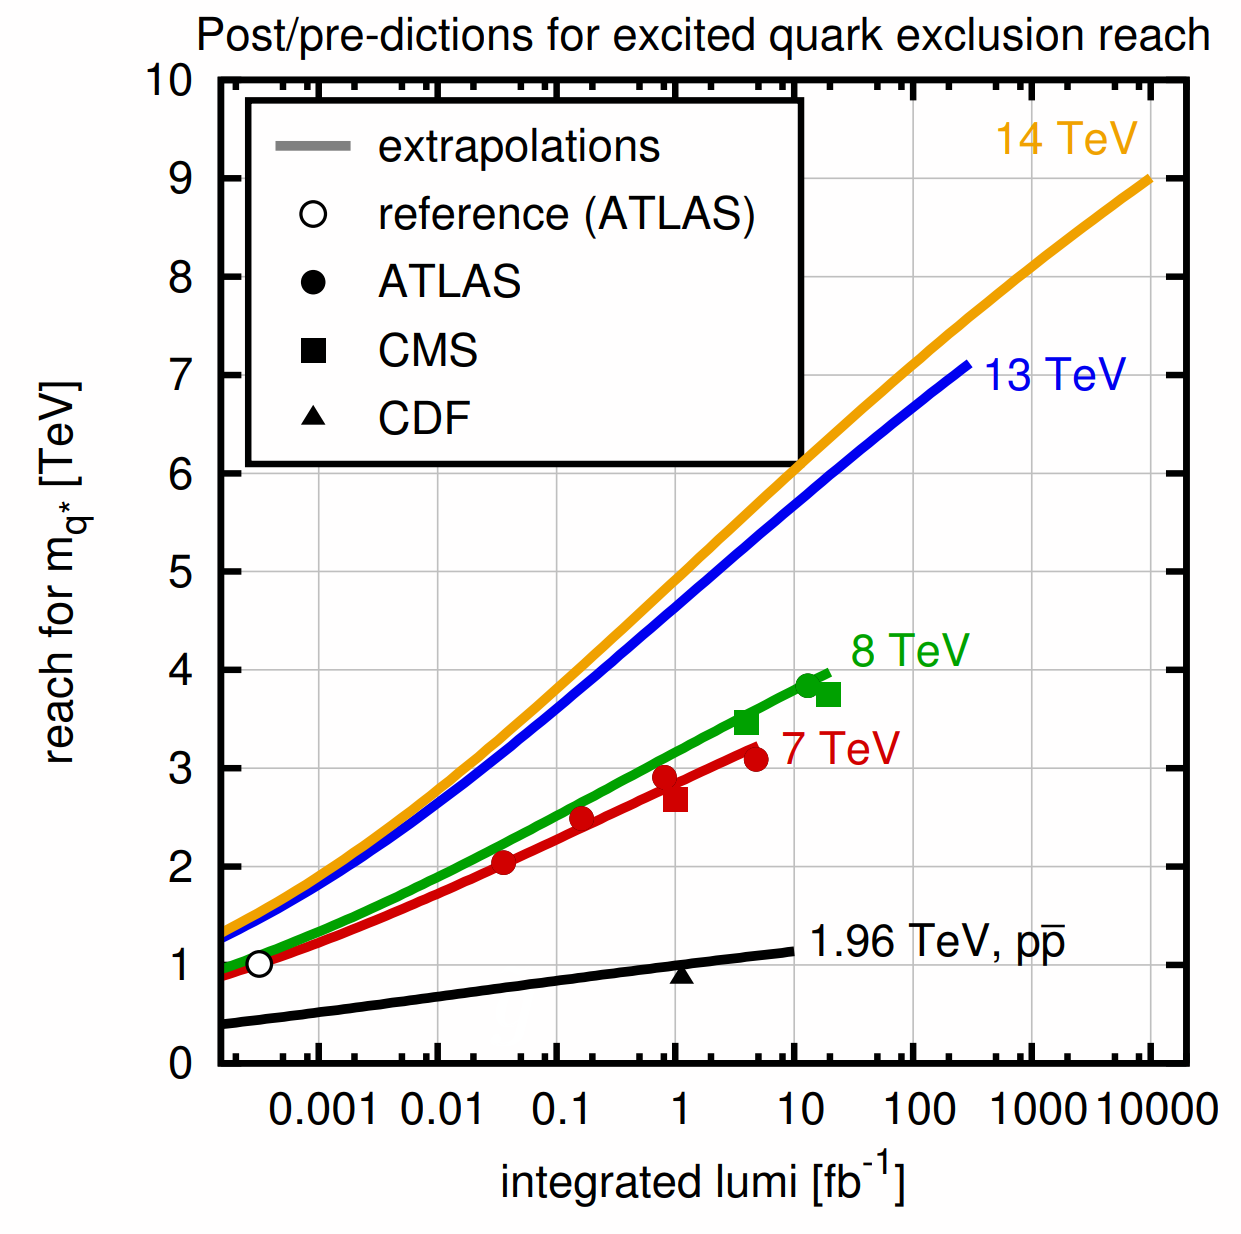
\includegraphics[width=0.7\columnwidth]{figures/Conclusion/QStarReach.png}
%	\caption{Predictions for the exclusion reach of dijet searches for excited quarks at the LHC for Run-1 and Run-2 energies and integrated luminosities.\cite{QStarReachSource}  Comparisons to published results for CDF and LHC Run 1 are shown in the filled shapes.}
%	\label{fig:QStarReach}
%\end{figure}
%
%\section{Benchmark Signals}
%
%The dijet search is designed to be as model-agnostic as possible, searching for $s$-channel production of a new resonance which decays to two quarks, two gluons, or one quark and one gluon.  Many possible models can describe this final state, of which a handful were chosen as benchmarks for this analysis.  These models are introduced here.  The goal of the analysis is not to discover or exclude certain models, but instead to provide results which can easily be interpreted in the context of other model-specific searches.
%
%\begin{figure}[]
%	\centering
%	\subfloat[]{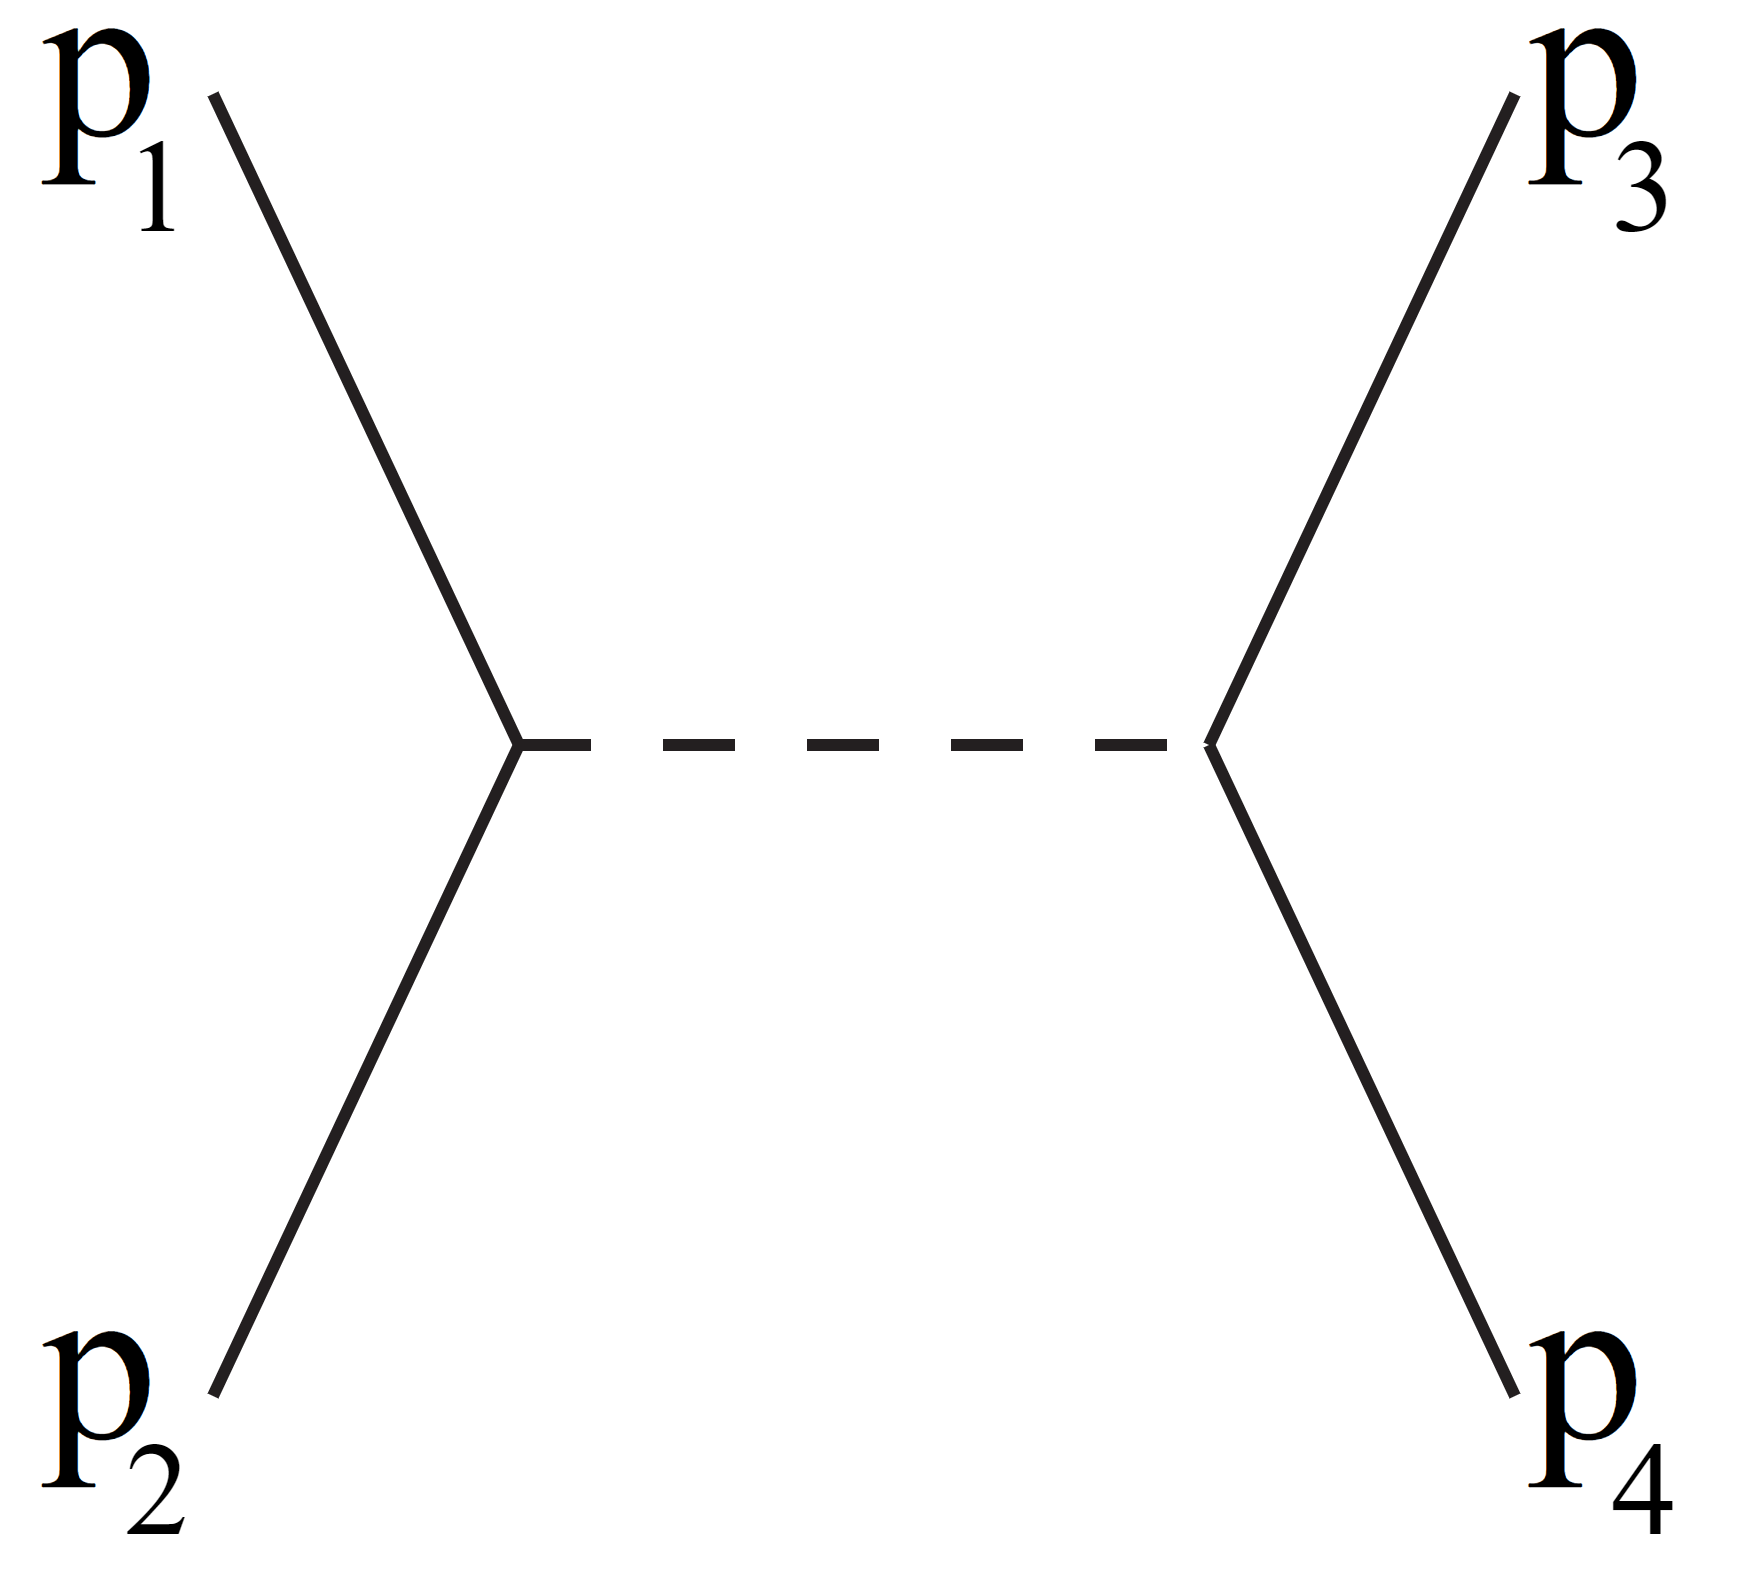
\includegraphics[width=0.35\columnwidth]{figures/Theory/SChannel.png}}
%	\hspace{0.1\columnwidth}%
%	\subfloat[]{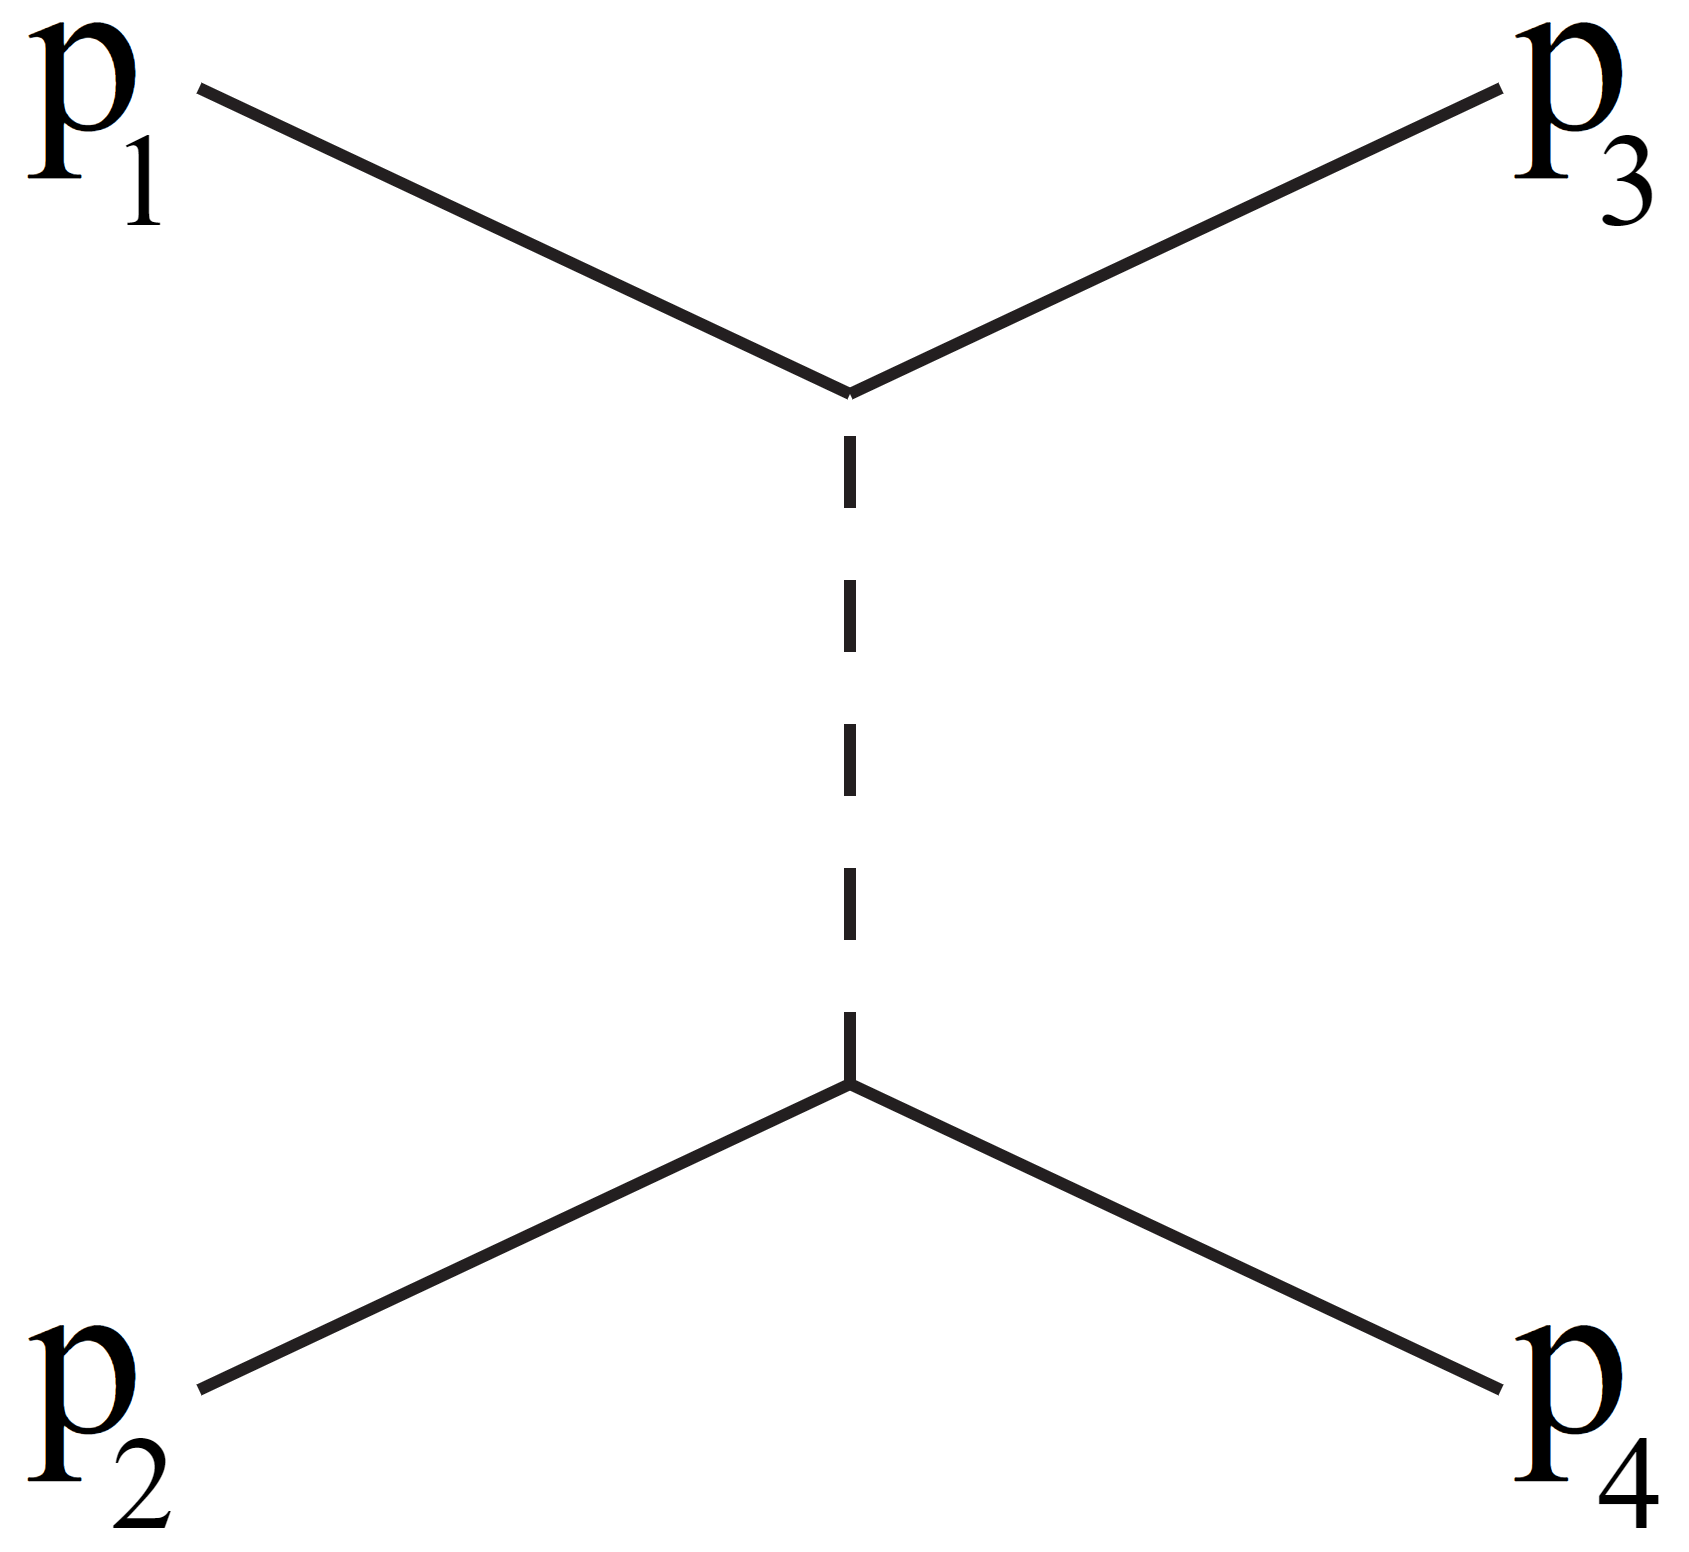
\includegraphics[width=0.35\columnwidth]{figures/Theory/TChannel.png}}
%	\caption{Feynman diagrams for (a) $s$-channel processes which could produce a new resonance and (b) $t$-channel background processes.
%	}
%	\label{fig:Feynman}
%\end{figure}
%
%\subsection{Excited Quarks}
%
%Excited quarks are a standard benchmark model for compositeness, where the quarks (and leptons) that we observe are not actually fundamental particles, but are made up of some smaller, unknown particles (typically called $preons$).  Composite models aim to address the mass hierarchy of the quarks and the patterns of fermion generations in the same way that the quark model explains the behavior of baryons and mesons.  Excited quark states would be produced around the scale of this new interaction.  In $pp$ collisions, a quark could be excited to a higher state through absorption of a gluon, and then radiate a boson as it returns to the ground state.  This search looks for evidence of a $q^* \rightarrow qg$ decay which corresponds to $\sim$85\% of the total branching ratio.  The other possible decay modes ($q^*\rightarrow\gamma,Z,W$) are not simulated and assumed to have zero acceptance in the search.
%
%The model used for the benchmark signal is described in Refs.~\cite{QStar} and \cite{QStar2}.  The parameters for the model are chosen such that the resonance has a relatively narrow width as shown in Figure~\ref{fig:QStarPeaks}.  If excited quarks are detectable at LHC energies, they should produce peaks which are very pronounced compared to the background QCD prediction.  The acceptance for the $q^*$ model is roughly flat as a function of mass, with low acceptance points in Figure~\ref{fig:QStarPeaks} being below the mass cut of the analysis.
%
%\begin{figure}[]
%	\centering
%	\subfloat[]{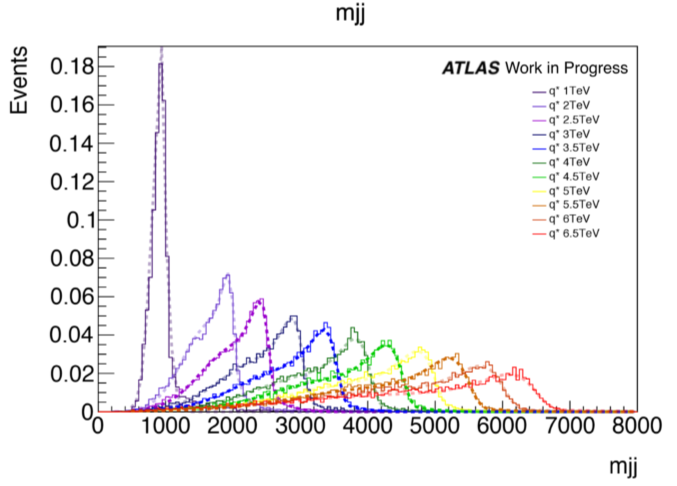
\includegraphics[width=0.51\columnwidth]{figures/Theory/QStarPeaks.png}}
%	\hspace{0.05\columnwidth}%
%	\subfloat[]{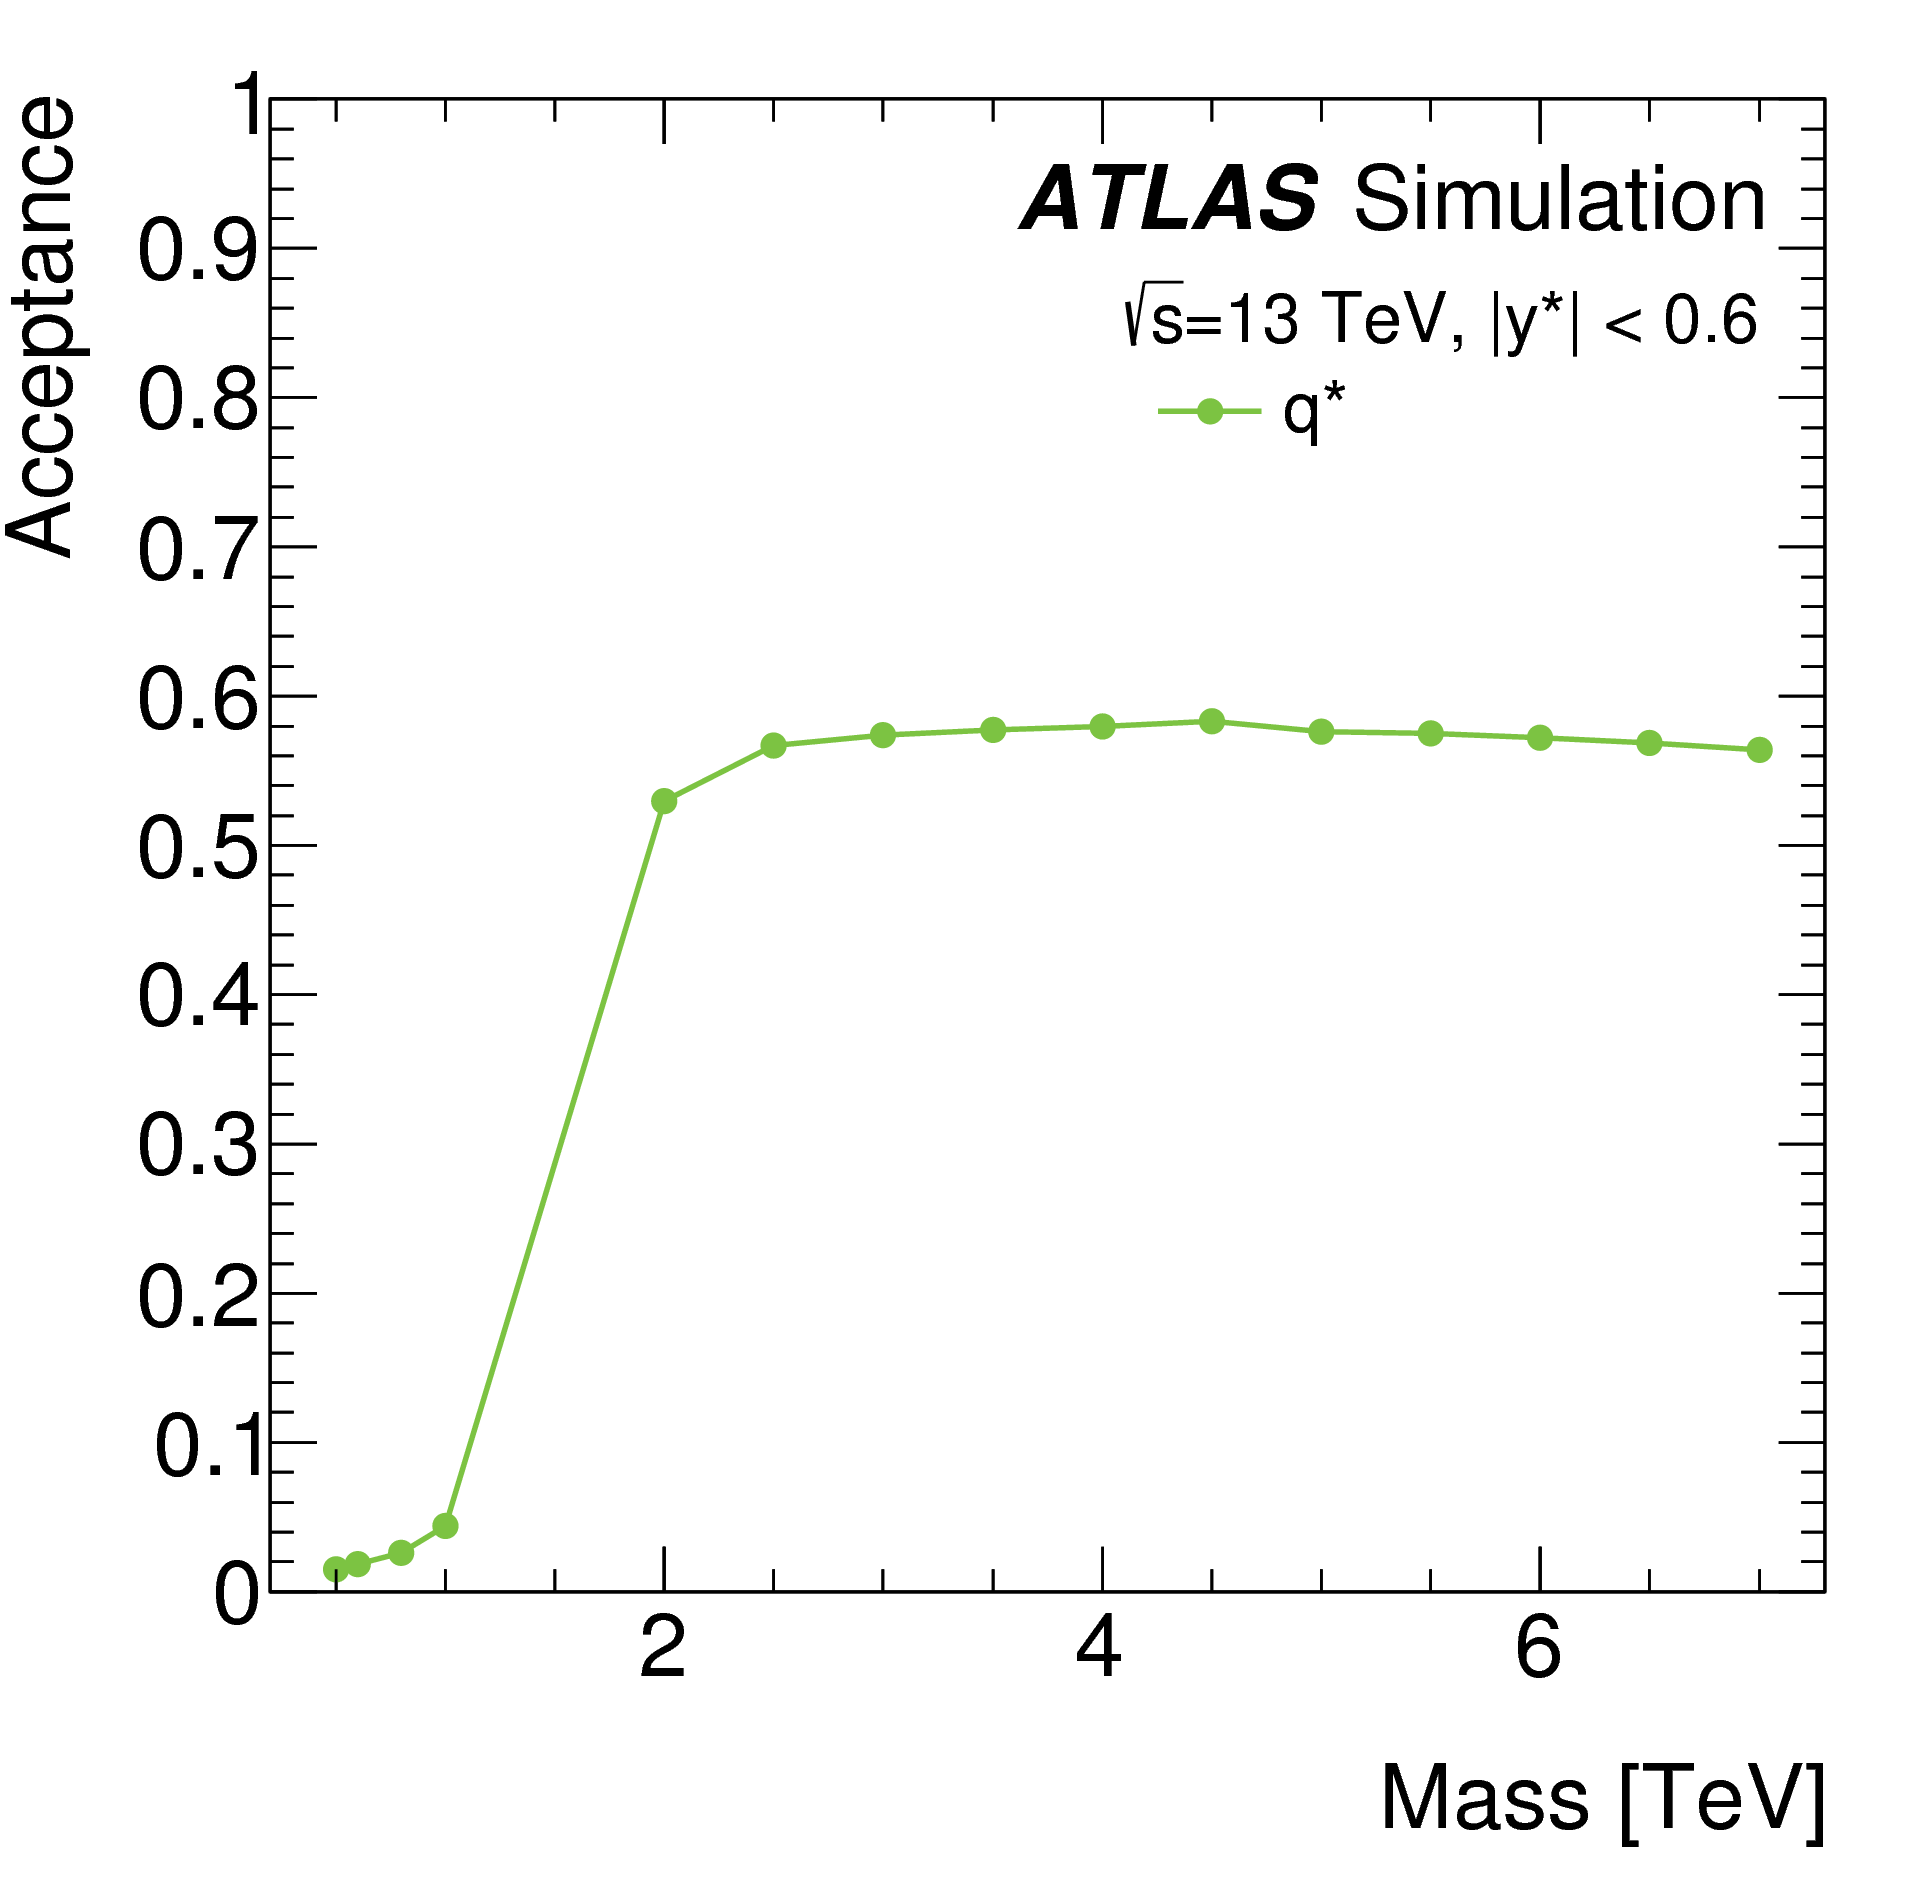
\includegraphics[width=0.34\columnwidth]{figures/Theory/QStarAcceptance.png}}
%	\caption{Truth level mass (a) and analysis acceptance (b) for $q^*$ samples at various mass points.  The acceptance is after the full analysis selection which is described in Chapter~\ref{ch:SearchStrategy}. 
%	}
%	\label{fig:QStarPeaks}
%\end{figure}
%
%\subsection{$W'$ Bosons}
%
%Many BSM theories which introduce additional W bosons are part of extended gauge theories.  The benchmark model used for this analysis is the Sequential Standard Model (SSM), where the $W'$ shares the same couplings as the SM $W$ boson, varying only in mass. The corresponding branching ratio to quark final states of 75\% from the process $W'\rightarrow qq$.  No interference between the $W'$ and the SM is simulated.
%
%In comparison to the $q^*$ signal, the $W'$ has a much more pronounced low-mass tail, as shown in Figure~\ref{fig:WPrimePeaks}.  As such, the acceptance for the model decreases significantly at higher mass points.
%
%\begin{figure}[]
%	\centering
%	\subfloat[]{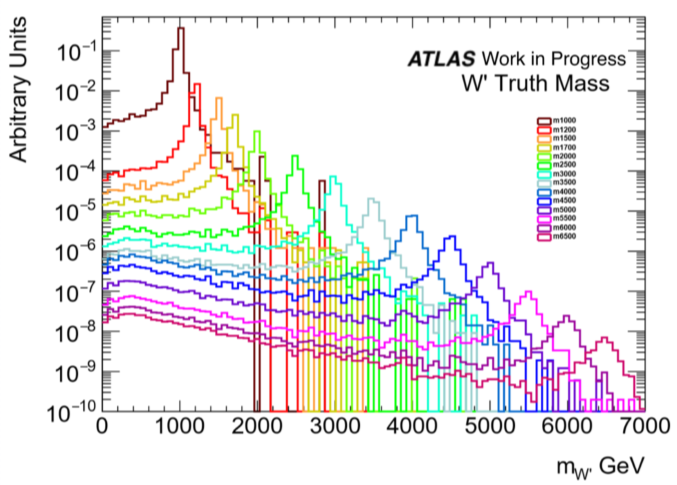
\includegraphics[width=0.49\columnwidth]{figures/Theory/WPrimePeaks.png}}
%	\hspace{0.05\columnwidth}%
%	\subfloat[]{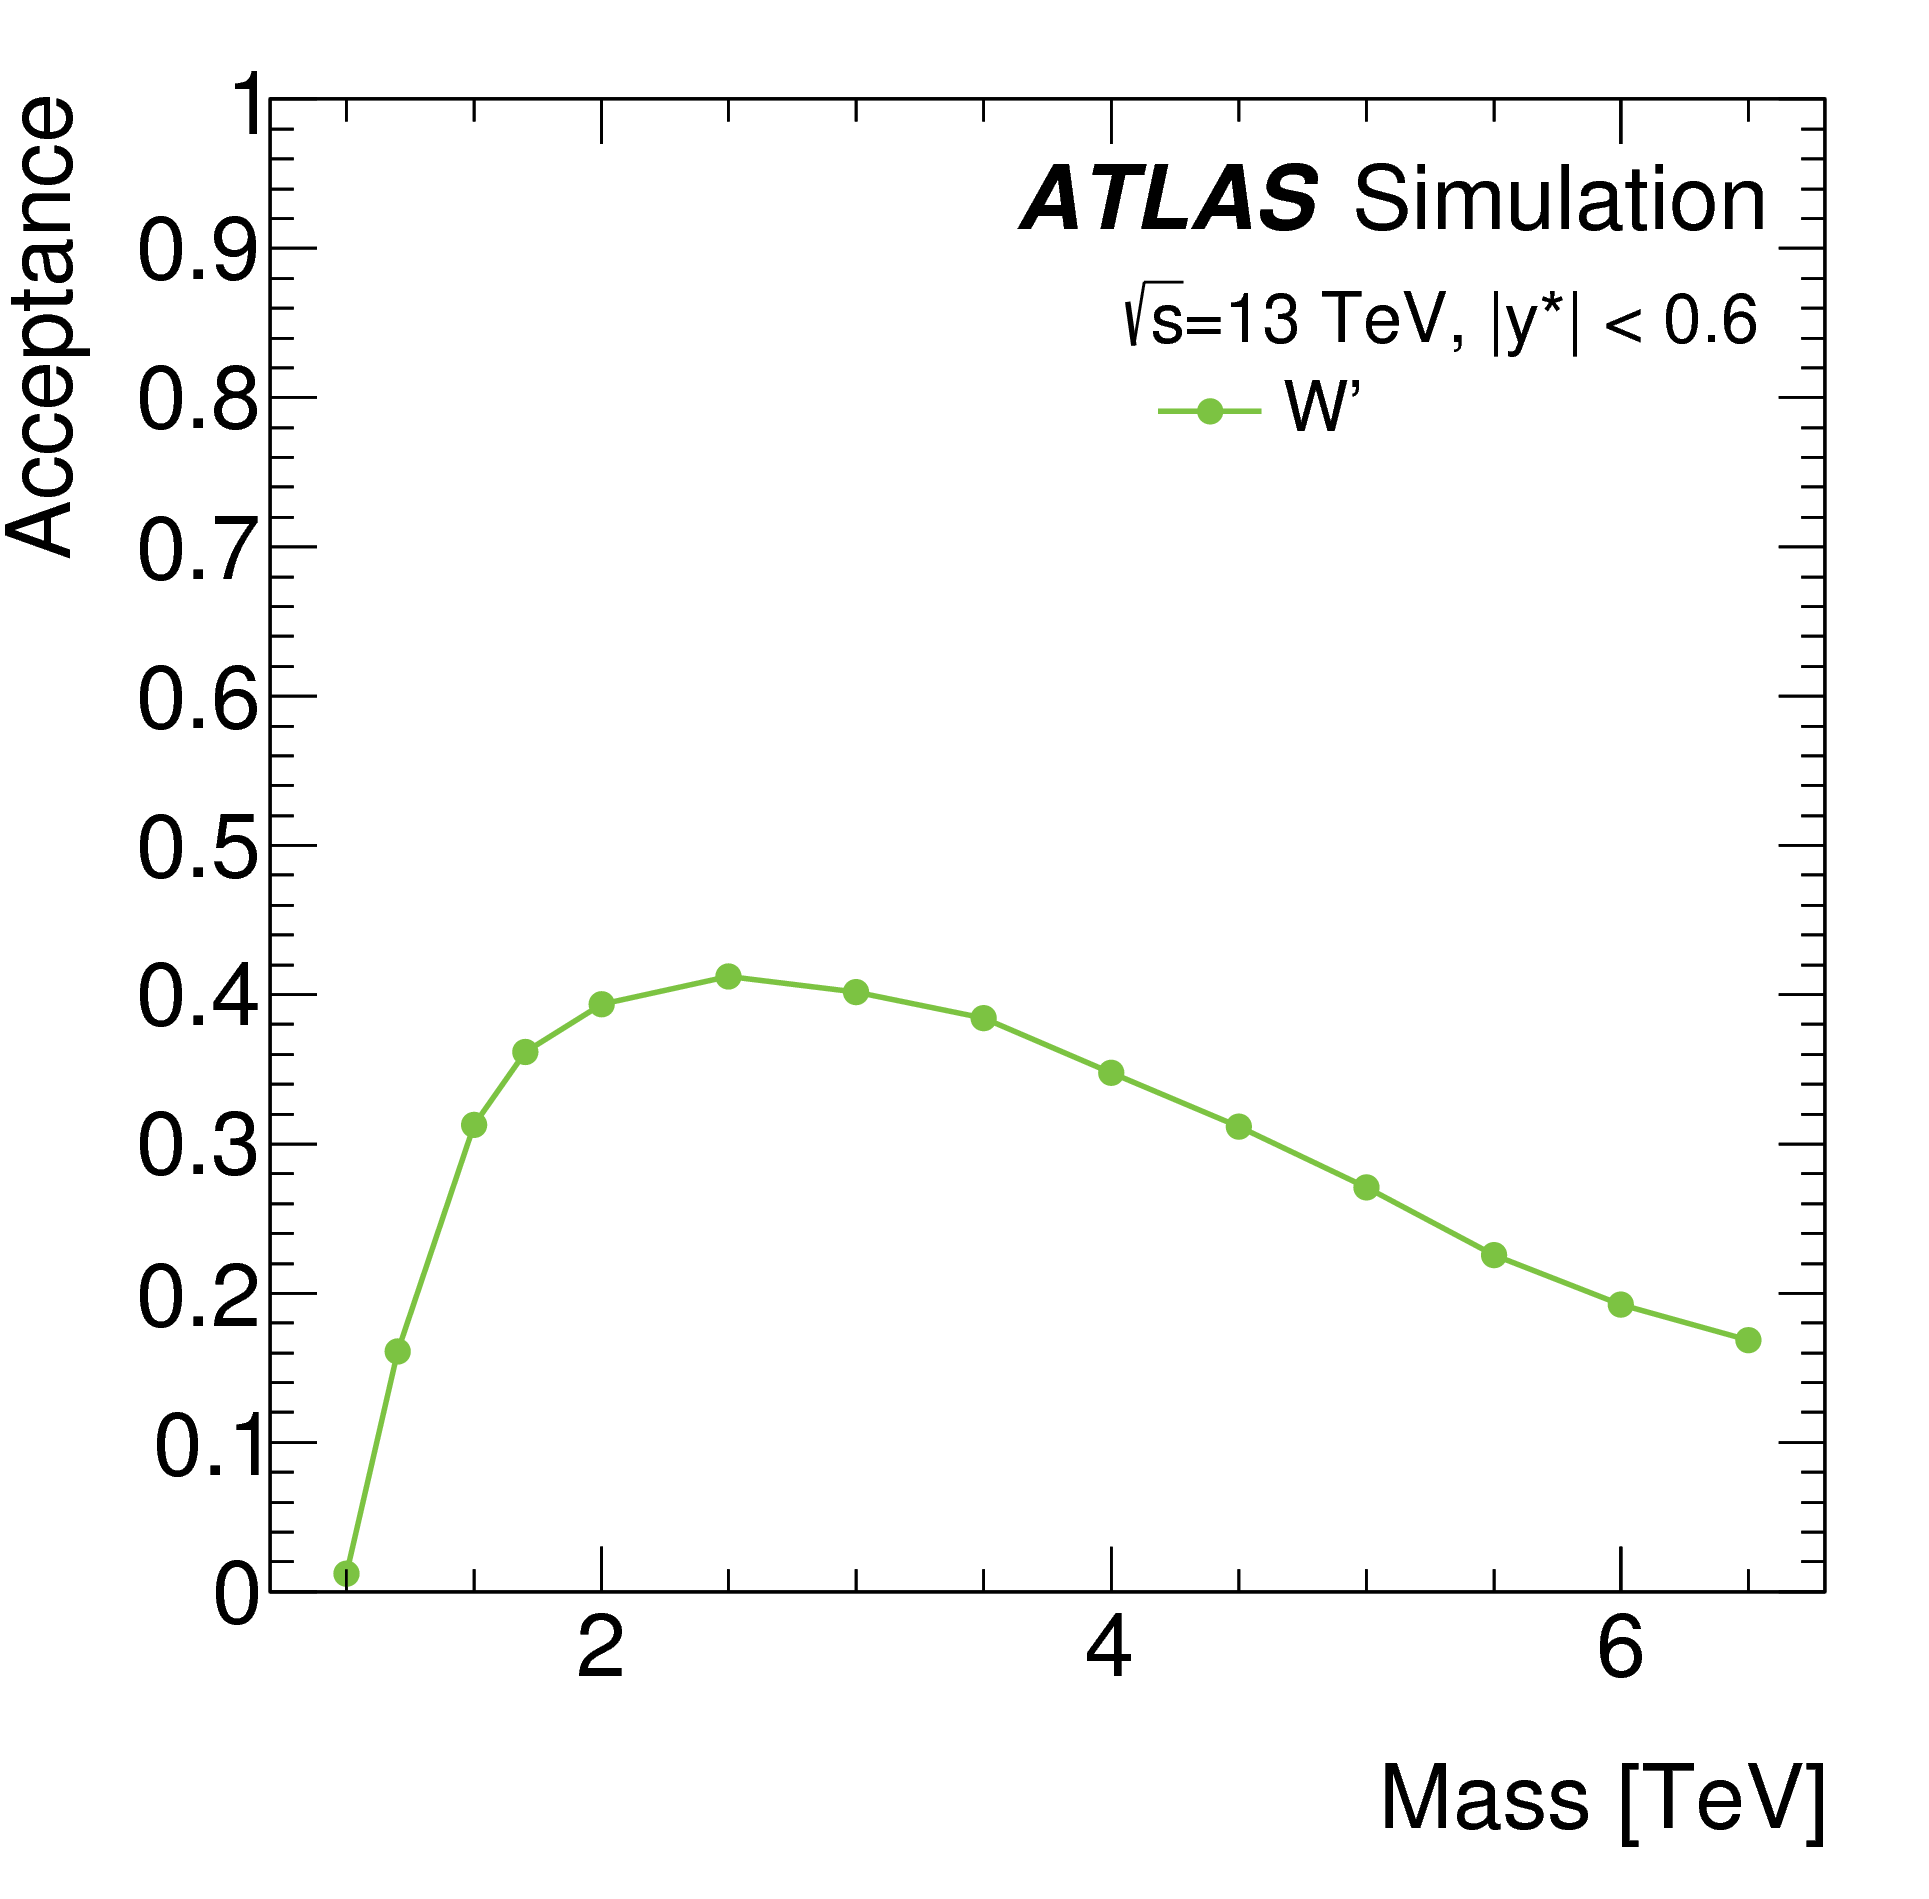
\includegraphics[width=0.36\columnwidth]{figures/Theory/WPrimeAcceptance.png}}
%	\caption{Truth level mass (a) and analysis acceptance (b) for $W'$ samples at various mass points.  The acceptance is after the full analysis selection which is described in Chapter~\ref{ch:SearchStrategy}.  The $W'$ signal points have a much larger low-mass tail, especially at high mass, due to significant off-shell production.
%	}
%	\label{fig:WPrimePeaks}
%\end{figure}
%
%\subsection{Excited W Bosons}
%
%Similar to an excited quark, an excited state of the W boson could point to compositeness there, with decays to a $qq$ final state.\cite{WStar}  Unlike all of the other models considered here, the angular distribution of $W^*$ decays do not peak at $y^*=|\eta_1-\eta_2|/2=0$, but rather at more forward angles, as shown in Figure~\ref{fig:WStarSignificance}.  As such, the $W^*$ search uses a separate second search region with a wider angular cut of $y^*<1.2$ to maximize signal significance.\cite{WStarTopology}
%
%The mixing angle $sin(\theta_X)$ determines the coupling to the quarks and leptons, for this particular model it is set to 0, creating a leptophobic state with maximal coupling to quarks, and thus the highest branching fraction to the dijet final state.  The coupling constants are selected in such a way to ensure that the $W^*$ has the same width as the $W'$ model used, helping to facilitate comparisons.   
%
%
%\begin{figure}[h!]
%	\centering
%	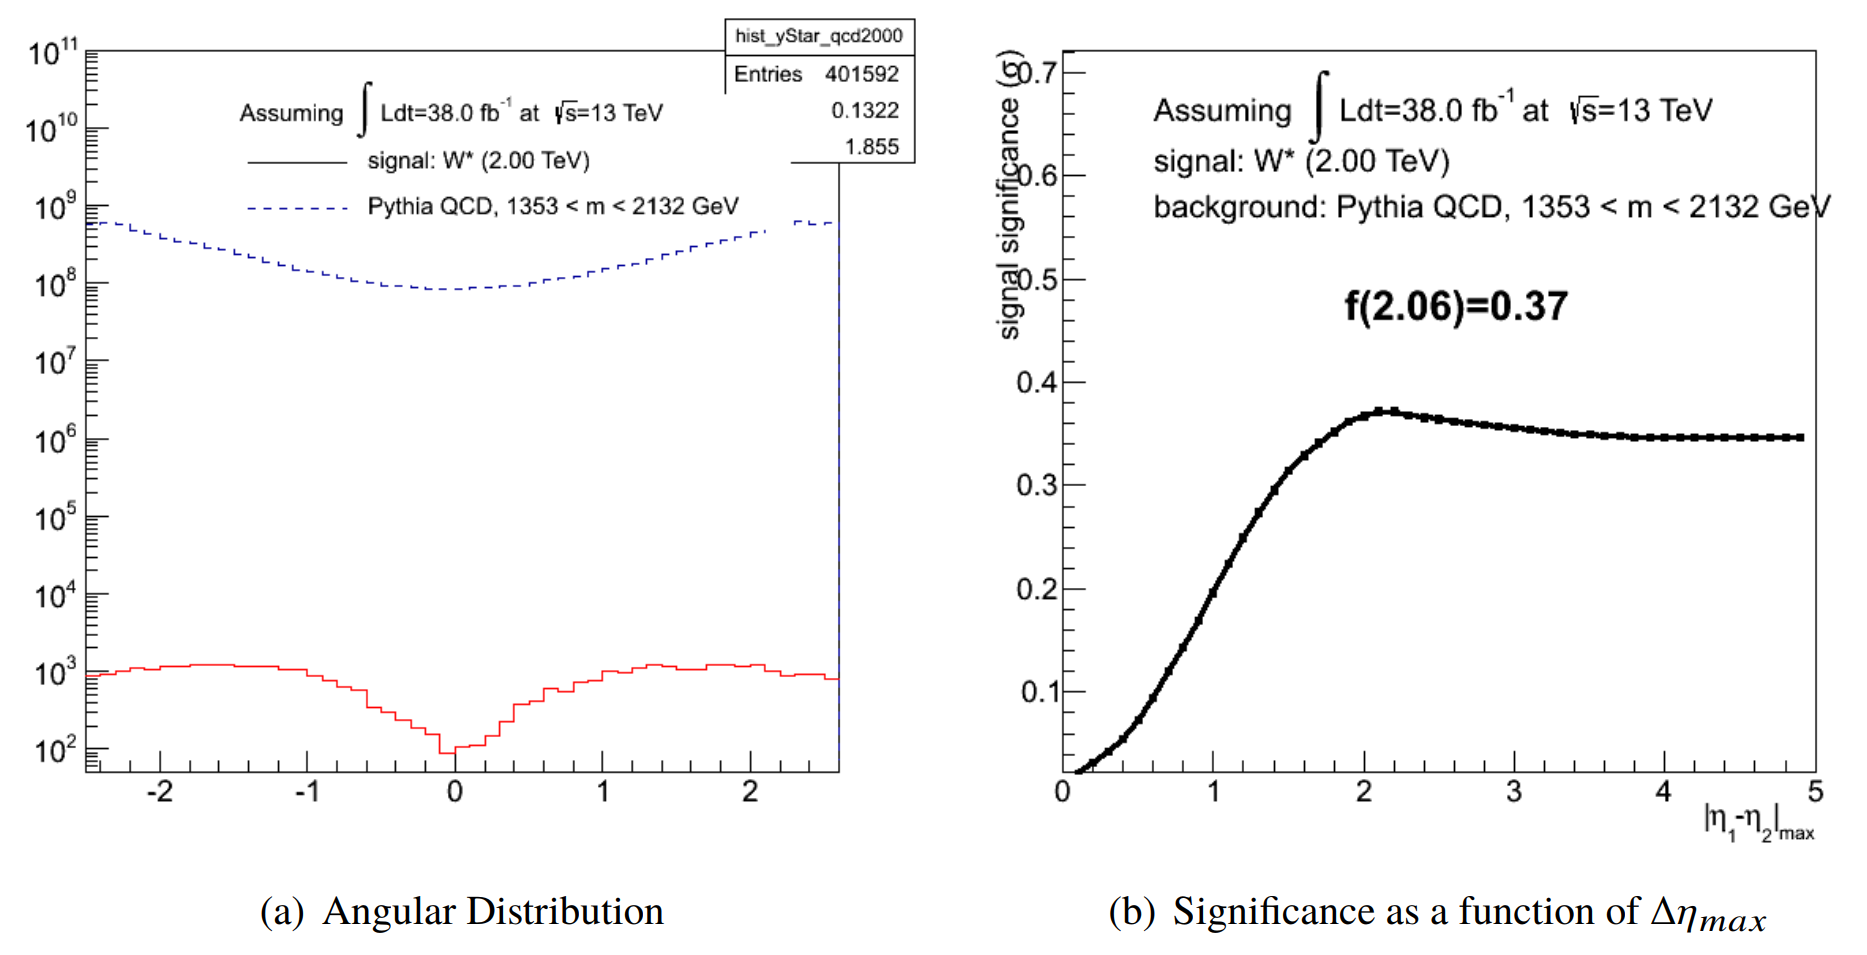
\includegraphics[width=\columnwidth]{figures/Theory/WStarSignificance.png}
%	\caption{(a) The angular distribution for the $W^*$ signal (red) compared to the QCD dijet background (blue).  (b) Signal significance as a function of angular cut.  The cut used in this analysis corresponds to a cut of 2.4 on the given plot.}
%	\label{fig:WStarSignificance}
%\end{figure}
%
%\subsection{$Z'$ Dark Matter Mediator}
%
%The existence of dark matter is extremely well motivated, from measurements of the rotation speeds of distant galaxies~\cite{DMGalaxy} to analyses of the cosmic microwave background.\cite{DMCMB}  Current estimates put the amount of dark matter at more than five times the amount of normal matter, yet there is no particle in the Standard Model that can explain this density.  A typical dark matter candidate interacts only with the weak and gravitational force; if it were charged under the EM or strong force it would be visible to us, or interact with regular matter in a detectable way.  These WIMPs (Weakly Interacting Massive Particles) are a feature of many BSM models, such as in R-parity conserving supersymmetry (SUSY) where the lightest stable SUSY particle does not decay and is uncharged.  Other models postulate a "dark sector" of particles which do not directly interact with regular matter, but instead have some mediator particle which couples to both the SM and dark matter.
%
%If there is some particle which couples to both Standard Model particles and the dark sector, then it could be produced at the LHC and be detected.  This search takes two different forms depending on the decay mode of the mediator.  If the mediator decays to the dark matter particle, it can be detected as missing transverse energy against a recoiling gluon or photon from initial state radiation.  If the mediator instead decays back into Standard Model particles, then its products could directly observed.  These two possible decays are shown in Figure~\ref{fig:ZPrimeFeynman}.
%
%
%\begin{figure}[]
%	\centering
%	\subfloat[]{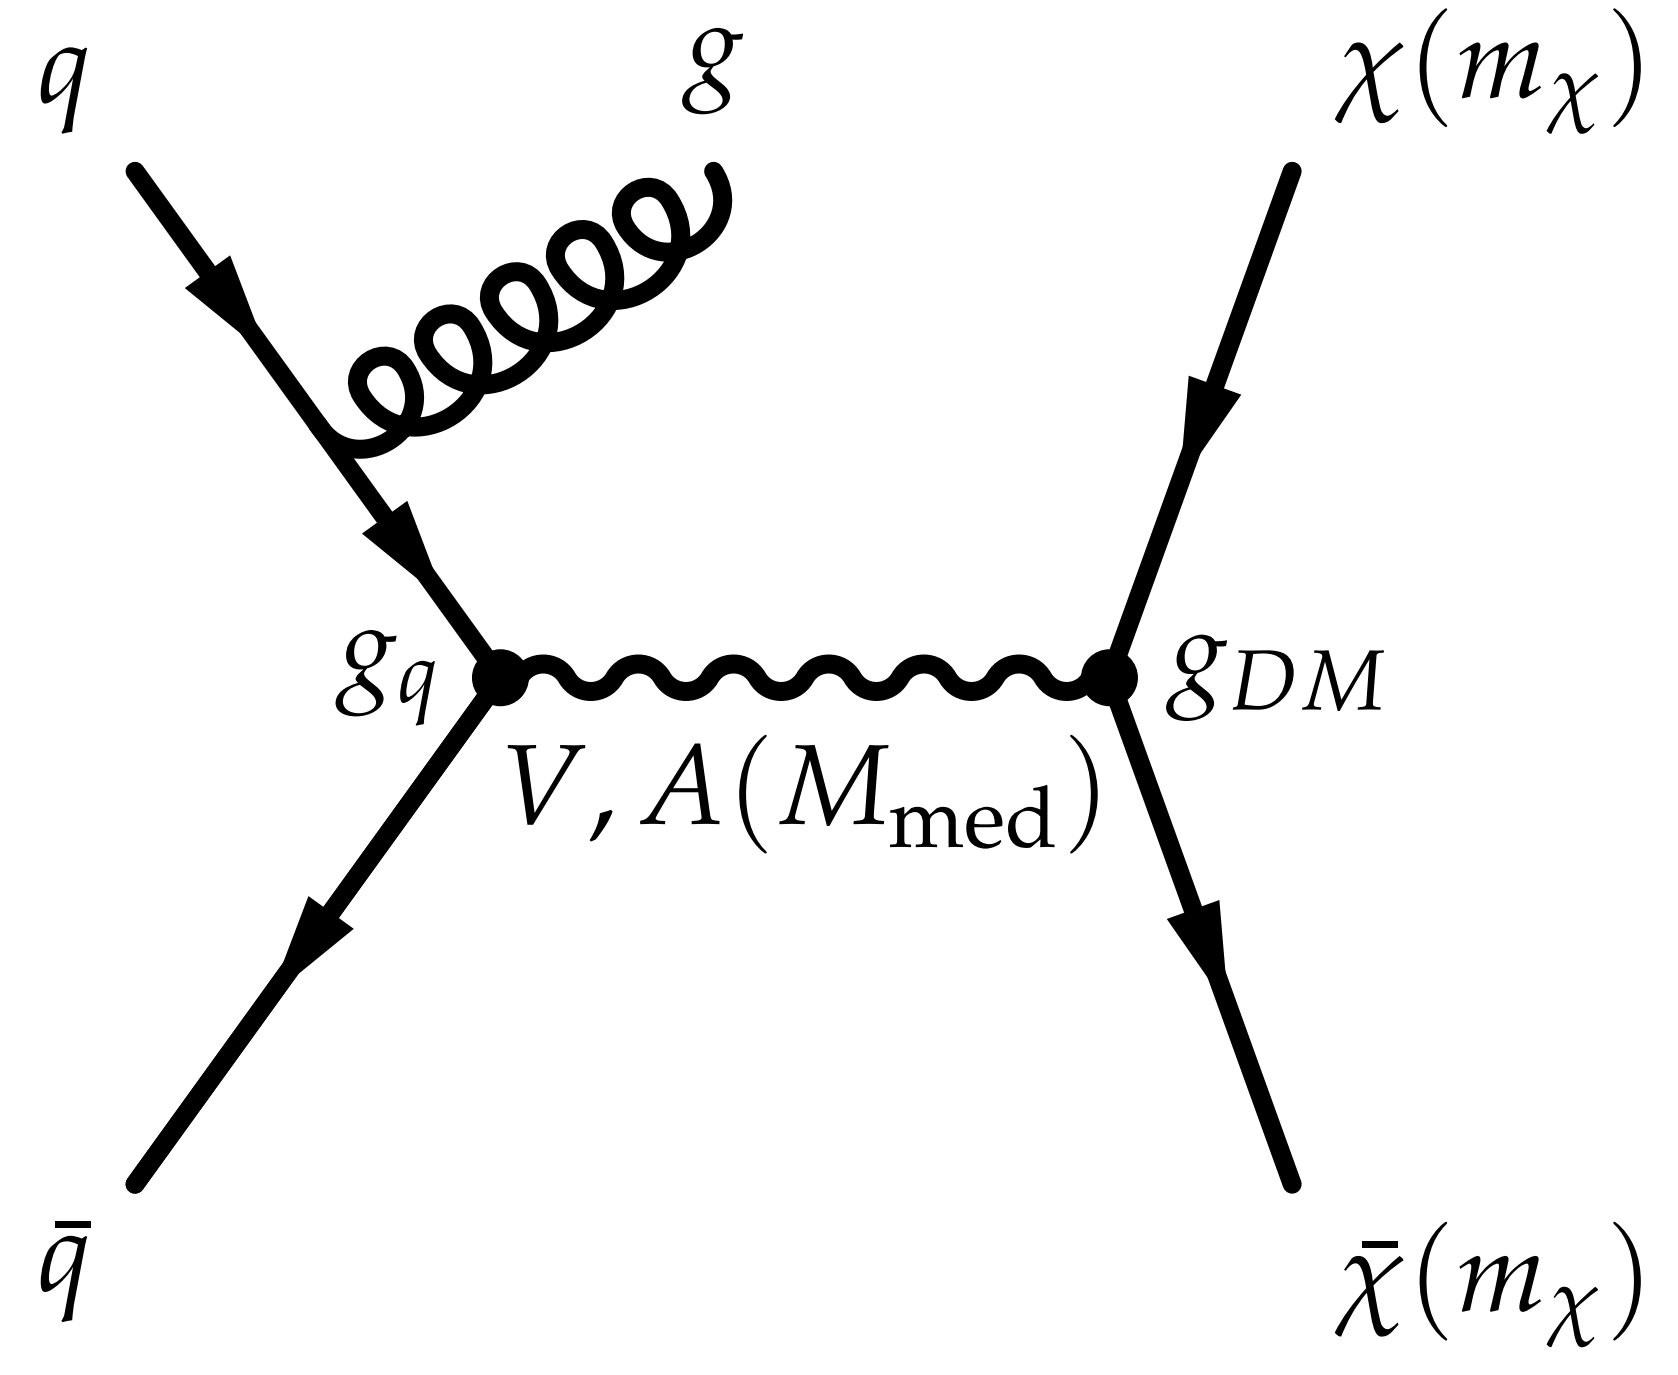
\includegraphics[width=0.45\columnwidth]{figures/Theory/MedToDM.png}\label{subfig:FeynmanMedToDM}}
%	\hspace{0.1\textwidth}%
%	\subfloat[]{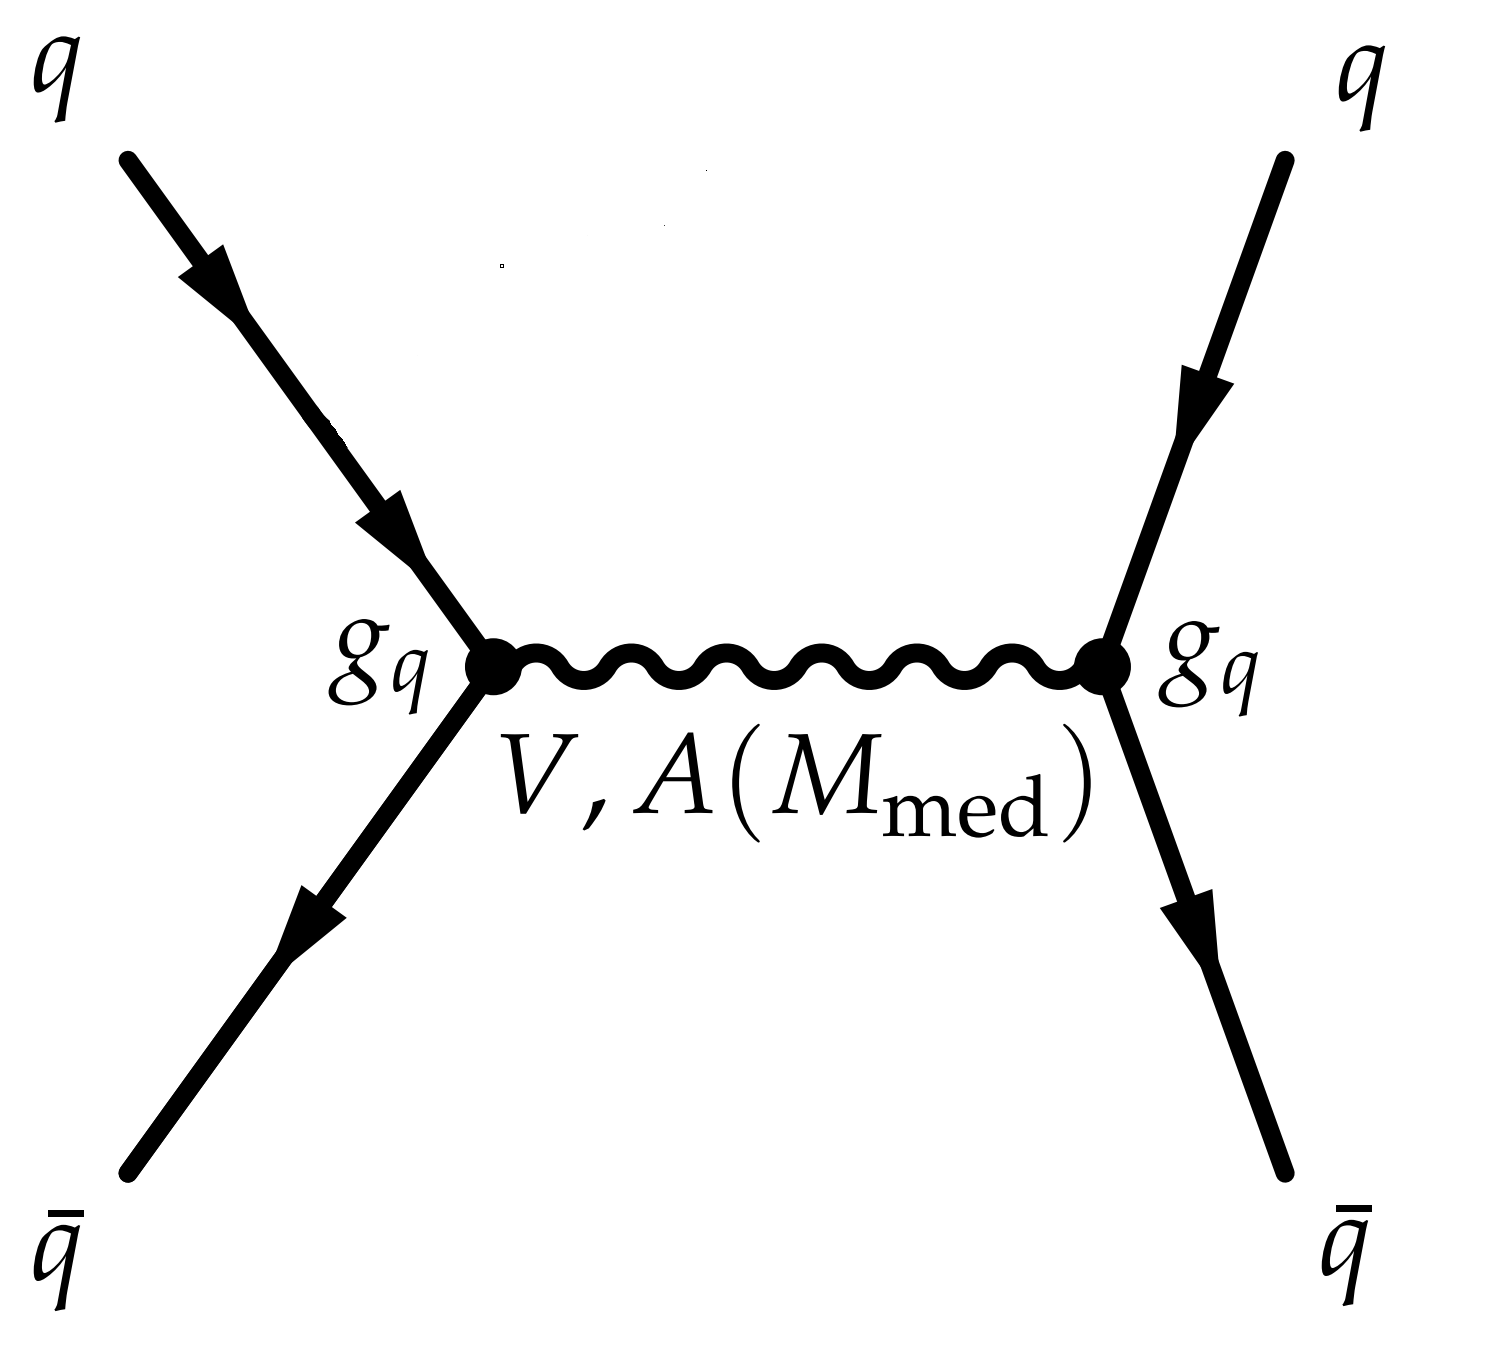
\includegraphics[width=0.41\columnwidth]{figures/Theory/MedToQQ.png}\label{subfig:FeynmanMedToQQ}}
%	\caption{Feynman diagrams for the $Z'$ decays searched for in the ATLAS dark matter mediator searches.  The cross-sections and kinematics depend upon the mediator and dark matter masses ($M_{med}, m_\chi$), and couplings to dark matter and quarks ($g_{DM}, g_q$). Diagrams similar to (a) are searched for using missing transverse energy along with initial state radiation, while (b) is the diagram of interest for the dijet search.
%	}
%	\label{fig:ZPrimeFeynman}
%\end{figure} 
%
%The $Z'$ model used is one of the benchmarks recommended by the ATLAS/CMS Dark Matter Forum~\cite{DMForum}, where the $Z'$ couples to dark matter, has axial-vector couplings to all SM quarks, and does not couple to leptons in any way.  The model then has four free parameters: $M_{med}$, the mediator mass, $m_\chi$, the mass of the dark matter particle, $g_q$, the coupling to quarks, and $g_{DM}$, the coupling to dark matter.  Both $m_\chi$ and $g_{DM}$ have second order effects on the behavior of the $Z'$ decays and are set to $M_{DM} = 10$\,TeV and $g_{DM} = 1.5$ respectively.  The relevant parameters are then the mediator mass, which sets the location of the excess, and $g_q$, which controls the decay cross-section and the width of the resonance.  Signal samples are generated for a range of masses and $g_q$.  Couplings beyond $g_q = 0.5$ are not considered as part of this analysis, as beyond this value the width of the resonance grows beyond 15\% and can no longer be properly detected by this search.  No interference with the SM is simulated.
%
%
%\subsection{Quantum Black Holes}
%
%In comparison to the other three fundamental forces, gravity is many, many orders of magnitude weaker.  The fundamental scale of gravity, the Planck mass ($m_P$), is equal to
%
%\begin{equation}
%m_P = \sqrt{\frac{\hbar c}{G}} = 1.22 \times 10^{19}\,\mathrm{GeV} / c^2
%\end{equation}
%where G is the gravitational constant.  This large gap between the scale of electroweak physics around 100\,GeV and the scale of gravity is known as the $hierarchy~problem$.  One possible solution to this issue is to postulate that gravity is around the same scale as the other forces, but that it is diluted into some number of extra spacial dimensions.  In the case of the ADD model (Arkani-Hamed, Dimopoulos, and Dvali)~\cite{ADD}, the 4-dimensional universe we observe is embedded in a higher-dimensional bulk spacetime where the extra dimensions are only accessible by gravitational fields.  Since the inverse-square law for gravity has been tested down to the sub-millimeter scale, these extra dimensions must be compact such that they have thus far escaped detection.
%
%If there are a number of such extra dimensions, the fundamental scale of gravity, $M_D$, could be low enough such that it could be accessible at LHC energies.  This introduces the possibility that microscopic or Quantum Black Holes (QBH) could be produced in proton-proton collisions.  If the black hole produced is well above $M_D$, it would quickly decay via Hawking radiation to a large number of particles, leaving behind a telltale high-multiplicity signature in the detector.  In the more likely scenario of a black hole being produced close to $M_D$, quantum effects dominate and a low-multiplicity final state is dominant.\cite{QBH}
%
%The particular benchmark model used is an ADD-type QBH with $n=6$ extra dimensions.  In this scenario, QBH produced near $M_D$ will decay to an average of two particles, and since it is created from the interaction of two strongly-charged partons, the decay to a two-parton final state is strongly favored.  The model used has an estimated branching ratio of 96\% to two partons.  As such, the final state looks very much like a new resonance produced near $M_D$ with a dijet final state, with a negligible low-mass tail and a signal width of approximately 10\%, as shown in Figure~\ref{fig:QBHPeaks}.
%
%\begin{figure}[]
%	\centering
%	\subfloat[]{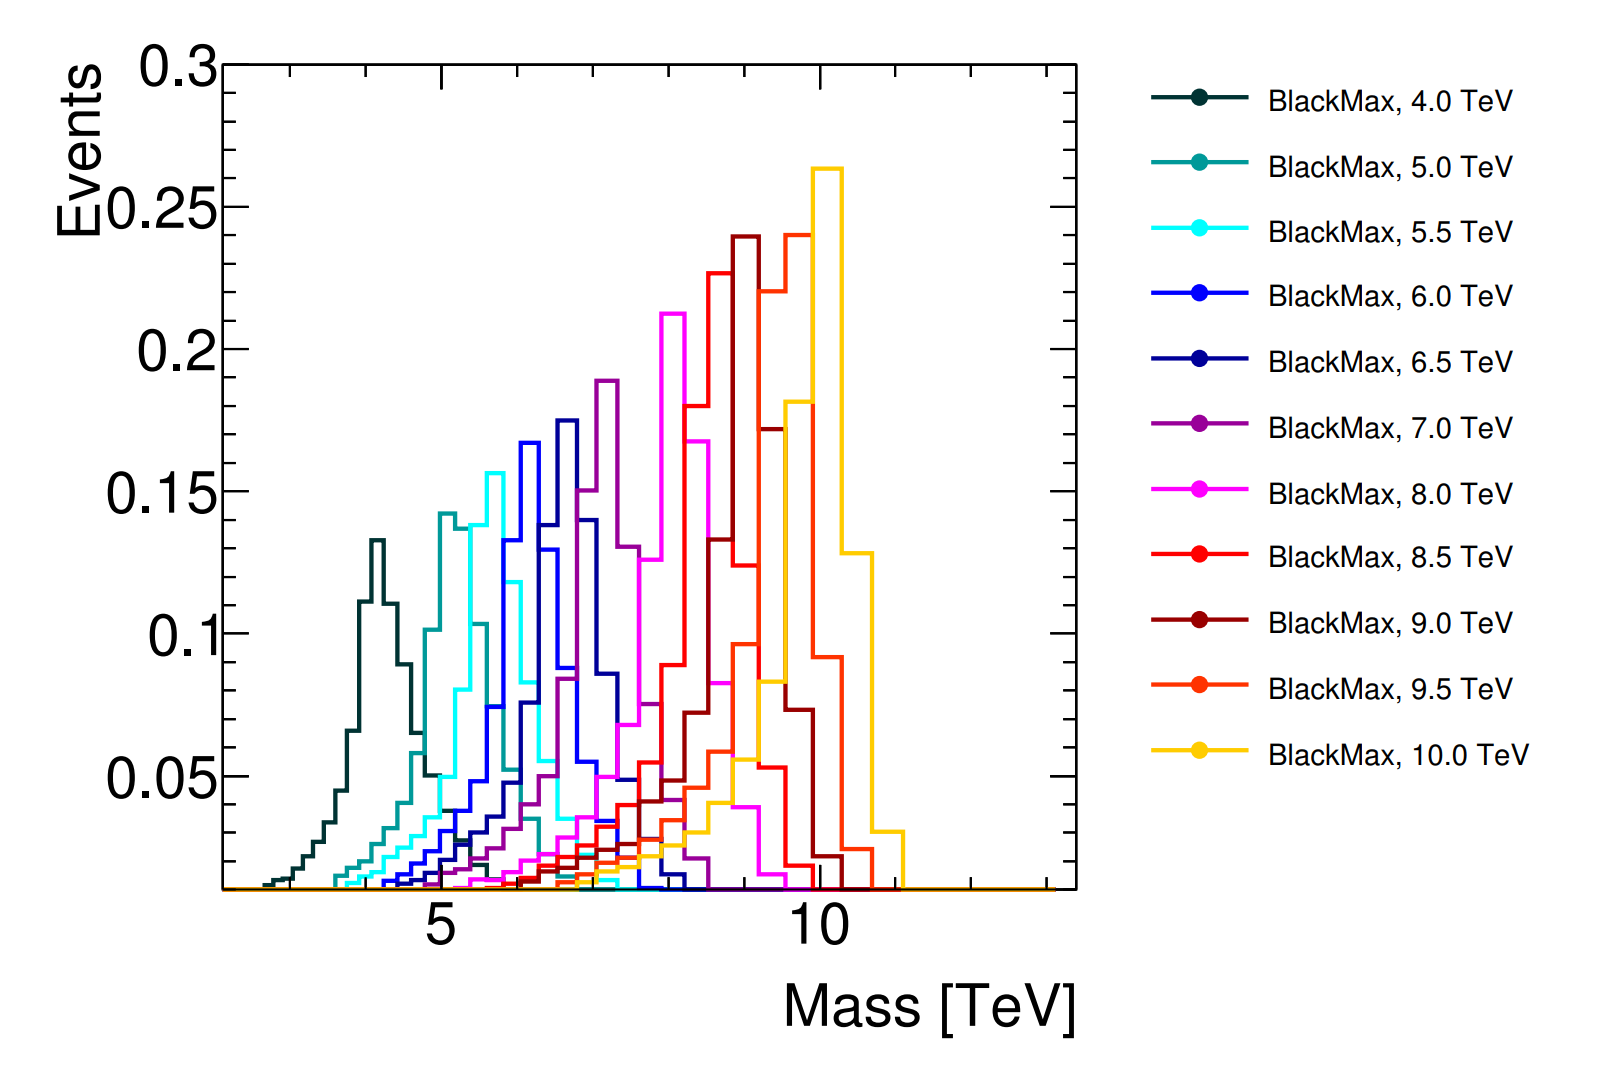
\includegraphics[width=0.51\columnwidth]{figures/Theory/QBHPeaks.png}}
%	\hspace{0.05\columnwidth}%
%	\subfloat[]{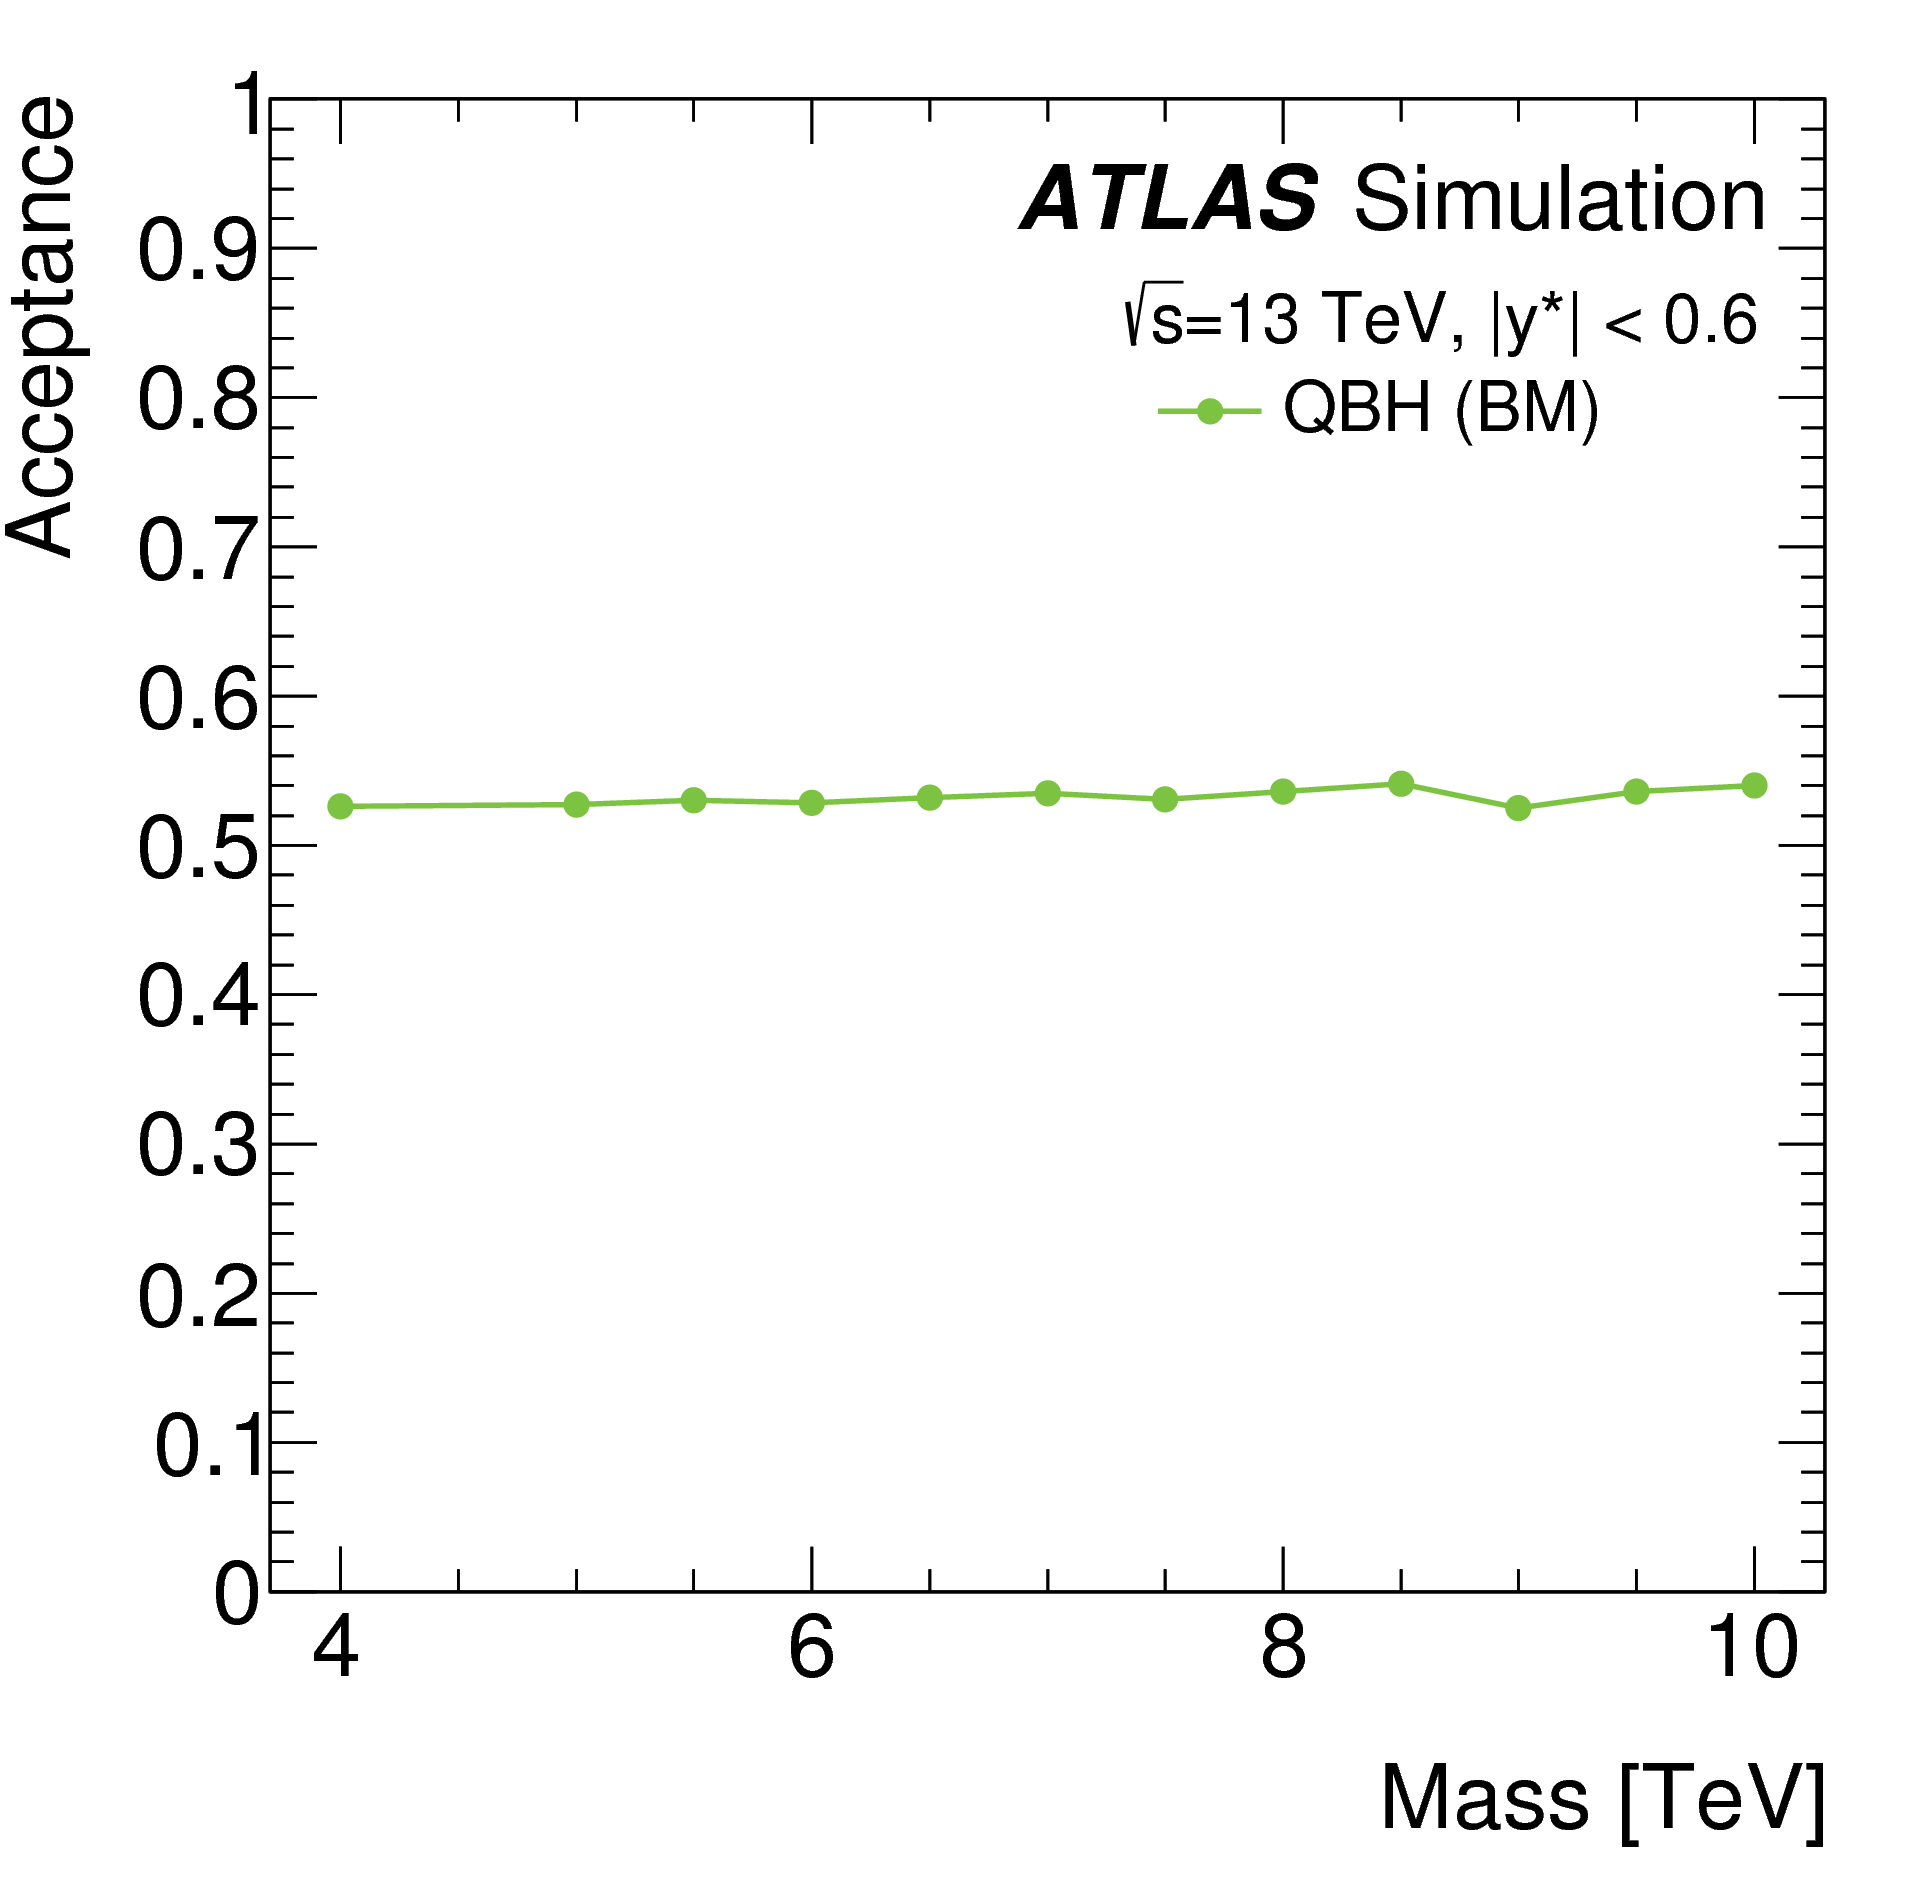
\includegraphics[width=0.34\columnwidth]{figures/Theory/QBHAcceptance.png}}
%	\caption{Truth level mass (a) and analysis acceptance (b) for QBH samples at various mass points.  The acceptance is after the full analysis selection which is described in Chapter~\ref{ch:SearchStrategy}. 
%	}
%	\label{fig:QBHPeaks}
%\end{figure}
